% Options for packages loaded elsewhere
\PassOptionsToPackage{unicode}{hyperref}
\PassOptionsToPackage{hyphens}{url}
\documentclass[
]{article}
\usepackage{xcolor}
\usepackage{amsmath,amssymb}
\setcounter{secnumdepth}{5}
\usepackage{iftex}
\ifPDFTeX
  \usepackage[T1]{fontenc}
  \usepackage[utf8]{inputenc}
  \usepackage{textcomp} % provide euro and other symbols
\else % if luatex or xetex
  \usepackage{unicode-math} % this also loads fontspec
  \defaultfontfeatures{Scale=MatchLowercase}
  \defaultfontfeatures[\rmfamily]{Ligatures=TeX,Scale=1}
\fi
% \usepackage{lmodern}
\ifPDFTeX\else
  % xetex/luatex font selection
\fi
% Use upquote if available, for straight quotes in verbatim environments
\IfFileExists{upquote.sty}{\usepackage{upquote}}{}
\IfFileExists{microtype.sty}{% use microtype if available
  \usepackage[]{microtype}
  \UseMicrotypeSet[protrusion]{basicmath} % disable protrusion for tt fonts
}{}
\makeatletter
\@ifundefined{KOMAClassName}{% if non-KOMA class
  \IfFileExists{parskip.sty}{%
    \usepackage{parskip}
  }{% else
    \setlength{\parindent}{0pt}
    \setlength{\parskip}{6pt plus 2pt minus 1pt}}
}{% if KOMA class
  \KOMAoptions{parskip=half}}
\makeatother
\usepackage{color}
\usepackage{fancyvrb}
\newcommand{\VerbBar}{|}
\newcommand{\VERB}{\Verb[commandchars=\\\{\}]}
\DefineVerbatimEnvironment{Highlighting}{Verbatim}{commandchars=\\\{\}}
% Add ',fontsize=\small' for more characters per line
\newenvironment{Shaded}{}{}
\newcommand{\AlertTok}[1]{\textcolor[rgb]{1.00,0.00,0.00}{\textbf{#1}}}
\newcommand{\AnnotationTok}[1]{\textcolor[rgb]{0.38,0.63,0.69}{\textbf{\textit{#1}}}}
\newcommand{\AttributeTok}[1]{\textcolor[rgb]{0.49,0.56,0.16}{#1}}
\newcommand{\BaseNTok}[1]{\textcolor[rgb]{0.25,0.63,0.44}{#1}}
\newcommand{\BuiltInTok}[1]{\textcolor[rgb]{0.00,0.50,0.00}{#1}}
\newcommand{\CharTok}[1]{\textcolor[rgb]{0.25,0.44,0.63}{#1}}
\newcommand{\CommentTok}[1]{\textcolor[rgb]{0.38,0.63,0.69}{\textit{#1}}}
\newcommand{\CommentVarTok}[1]{\textcolor[rgb]{0.38,0.63,0.69}{\textbf{\textit{#1}}}}
\newcommand{\ConstantTok}[1]{\textcolor[rgb]{0.53,0.00,0.00}{#1}}
\newcommand{\ControlFlowTok}[1]{\textcolor[rgb]{0.00,0.44,0.13}{\textbf{#1}}}
\newcommand{\DataTypeTok}[1]{\textcolor[rgb]{0.56,0.13,0.00}{#1}}
\newcommand{\DecValTok}[1]{\textcolor[rgb]{0.25,0.63,0.44}{#1}}
\newcommand{\DocumentationTok}[1]{\textcolor[rgb]{0.73,0.13,0.13}{\textit{#1}}}
\newcommand{\ErrorTok}[1]{\textcolor[rgb]{1.00,0.00,0.00}{\textbf{#1}}}
\newcommand{\ExtensionTok}[1]{#1}
\newcommand{\FloatTok}[1]{\textcolor[rgb]{0.25,0.63,0.44}{#1}}
\newcommand{\FunctionTok}[1]{\textcolor[rgb]{0.02,0.16,0.49}{#1}}
\newcommand{\ImportTok}[1]{\textcolor[rgb]{0.00,0.50,0.00}{\textbf{#1}}}
\newcommand{\InformationTok}[1]{\textcolor[rgb]{0.38,0.63,0.69}{\textbf{\textit{#1}}}}
\newcommand{\KeywordTok}[1]{\textcolor[rgb]{0.00,0.44,0.13}{\textbf{#1}}}
\newcommand{\NormalTok}[1]{#1}
\newcommand{\OperatorTok}[1]{\textcolor[rgb]{0.40,0.40,0.40}{#1}}
\newcommand{\OtherTok}[1]{\textcolor[rgb]{0.00,0.44,0.13}{#1}}
\newcommand{\PreprocessorTok}[1]{\textcolor[rgb]{0.74,0.48,0.00}{#1}}
\newcommand{\RegionMarkerTok}[1]{#1}
\newcommand{\SpecialCharTok}[1]{\textcolor[rgb]{0.25,0.44,0.63}{#1}}
\newcommand{\SpecialStringTok}[1]{\textcolor[rgb]{0.73,0.40,0.53}{#1}}
\newcommand{\StringTok}[1]{\textcolor[rgb]{0.25,0.44,0.63}{#1}}
\newcommand{\VariableTok}[1]{\textcolor[rgb]{0.10,0.09,0.49}{#1}}
\newcommand{\VerbatimStringTok}[1]{\textcolor[rgb]{0.25,0.44,0.63}{#1}}
\newcommand{\WarningTok}[1]{\textcolor[rgb]{0.38,0.63,0.69}{\textbf{\textit{#1}}}}
\usepackage{longtable,booktabs,array}
\newcounter{none} % for unnumbered tables
\usepackage{calc} % for calculating minipage widths
% Correct order of tables after \paragraph or \subparagraph
\usepackage{etoolbox}
\makeatletter
\patchcmd\longtable{\par}{\if@noskipsec\mbox{}\fi\par}{}{}
\makeatother
% Allow footnotes in longtable head/foot
\IfFileExists{footnotehyper.sty}{\usepackage{footnotehyper}}{\usepackage{footnote}}
\makesavenoteenv{longtable}
\usepackage{graphicx}
\makeatletter
\newsavebox\pandoc@box
\newcommand*\pandocbounded[1]{% scales image to fit in text height/width
  \sbox\pandoc@box{#1}%
  \Gscale@div\@tempa{\textheight}{\dimexpr\ht\pandoc@box+\dp\pandoc@box\relax}%
  \Gscale@div\@tempb{\linewidth}{\wd\pandoc@box}%
  \ifdim\@tempb\p@<\@tempa\p@\let\@tempa\@tempb\fi% select the smaller of both
  \ifdim\@tempa\p@<\p@\scalebox{\@tempa}{\usebox\pandoc@box}%
  \else\usebox{\pandoc@box}%
  \fi%
}
% Set default figure placement to htbp
\def\fps@figure{htbp}
\makeatother
\setlength{\emergencystretch}{3em} % prevent overfull lines
\providecommand{\tightlist}{%
  \setlength{\itemsep}{0pt}\setlength{\parskip}{0pt}}
\usepackage[]{natbib}
\bibliographystyle{plainnat}
\makeatletter
\@ifpackageloaded{subcaption}{}{\usepackage{subcaption}}
\@ifpackageloaded{caption}{}{\usepackage{caption}}
\captionsetup[subfigure]{margin=0.5em}
\AtBeginDocument{%
\renewcommand*\figurename{Figure}
\renewcommand*\tablename{Table}
}
\AtBeginDocument{%
\renewcommand*\listfigurename{List of Figures}
\renewcommand*\listtablename{List of Tables}
}
\newcounter{pandoccrossref@subfigures@footnote@counter}
\newenvironment{pandoccrossrefsubfigures}{%
\setcounter{pandoccrossref@subfigures@footnote@counter}{0}
\begin{figure}\centering%
\gdef\global@pandoccrossref@subfigures@footnotes{}%
\DeclareRobustCommand{\footnote}[1]{\footnotemark%
\stepcounter{pandoccrossref@subfigures@footnote@counter}%
\ifx\global@pandoccrossref@subfigures@footnotes\empty%
\gdef\global@pandoccrossref@subfigures@footnotes{{##1}}%
\else%
\g@addto@macro\global@pandoccrossref@subfigures@footnotes{, {##1}}%
\fi}}%
{\end{figure}%
\addtocounter{footnote}{-\value{pandoccrossref@subfigures@footnote@counter}}
\@for\f:=\global@pandoccrossref@subfigures@footnotes\do{\stepcounter{footnote}\footnotetext{\f}}%
\gdef\global@pandoccrossref@subfigures@footnotes{}}
\@ifpackageloaded{float}{}{\usepackage{float}}
\floatstyle{ruled}
\@ifundefined{c@chapter}{\newfloat{codelisting}{h}{lop}}{\newfloat{codelisting}{h}{lop}[chapter]}
\floatname{codelisting}{Listing}
\newcommand*\listoflistings{\listof{codelisting}{List of Listings}}
\makeatother
\usepackage{bookmark}
\IfFileExists{xurl.sty}{\usepackage{xurl}}{} % add URL line breaks if available
\urlstyle{same}
% fallback for those not using the hyperref driver hyperxmp:
\makeatletter
\@ifundefined{xmpquote}{\newcommand{\xmpquote}[1]{#1}}{}
\makeatother
\hypersetup{
  colorlinks=true,linkcolor=red,urlcolor=red,citecolor=red,anchorcolor=red,filecolor=red,
  pdfcreator={LaTeX via pandoc}}

\author{}
\date{}

\IfFileExists{seqsplit.sty}{\usepackage{seqsplit}}{\newcommand{\seqsplit}[1]{#1}}
\protected\def\breakseq#1{\seqsplit{#1}}
\protected\def\breaktt#1{\begingroup\ttfamily\seqsplit{#1}\endgroup}
\title{Refinement of Gold: A Metallurgical Analogy for Scientific Manuscript Composition}
\author{Daniel Ari Friedman\\\footnotesize{Active Inference Institute}\\\footnotesize{\texttt{daniel@activeinference.institute}}\\\footnotesize{\href{https://orcid.org/0000-0001-6232-9096}{ORCID: 0000-0001-6232-9096}} \\ \footnotesize{DOI: \href{https://doi.org/10.5281/zenodo.20931955}{10.5281/zenodo.20931955}}}
\date{2026-06-25}

% Core mathematics
\usepackage{amsmath}
\usepackage{amssymb}
\usepackage{amsfonts}
\usepackage{amsthm}

% Document layout
\usepackage{geometry}
\geometry{margin=0.25in}
\usepackage{float}
\usepackage{graphicx}

% Tables
\usepackage{booktabs}
\usepackage{longtable}
\usepackage{array}

% Typography and formatting
\usepackage{microtype}
\usepackage{xcolor}

% Cross-references and citations
\usepackage{hyperref}
\hypersetup{
    colorlinks=true,
    allcolors=red
}
\usepackage[capitalise,noabbrev]{cleveref}
\usepackage{natbib}

\begin{document}

\begin{titlepage}
\centering
\vspace*{2cm}
{\LARGE\bfseries Refinement of Gold: A Metallurgical Analogy for Scientific Manuscript Composition\par}
\vspace{0.75em}
{\large From Ore to Nine-Nines Purity via Mega-Madlib Token Injection\par}
\vfill
\makeatletter
{\@author\par}
\vspace{1em}
{\@date\par}
\makeatother
\vfill
\end{titlepage}
\thispagestyle{empty}
\tableofcontents
\newpage


\section{Abstract}\label{sec:abstract}

This paper presents a metallurgical analogy for scientific manuscript
composition, mapping gold-refining stages onto the template
infrastructure pipeline. The refinery processes manuscript ore through 5
stages --- from raw draft (9K, about 37.5\% purity) through
smelting, assaying, and cupellation --- to nine-nines certification
(99.9999999\%), the ultra-high-purity standard of electronics-grade
gold.

The analogy is \textbf{load-bearing}, not merely rhetorical: each
metallurgical stage corresponds to a real template-infrastructure
operation. Smelting removes dross (filler, unsupported claims); assaying
tests claims against evidence; cupellation resolves cross-references;
certification validates the full pipeline. The mega-madlib token engine
selects 24 domain tokens deterministically via seeded SHA-256 digest
over category inventories, ensuring every prose element is traceable and
reproducible.

The contribution is also formalized: 6 equation-backed formalisms define
purity, monotone refinement, token selection, claim support, gate
vectors, and certification. The project-local claim assay reports 8/8
supported contribution claims (100.00\%, passing), while the integrity
model exposes 8 source-owned risk dimensions and the shared template
evidence registry contributes 230 source-tiered facts when the
validation gate has run.

\textbf{Results:} The refinery achieves final purity of 99.9999999\%
(nine-nines) (24K (nine-nines certified)) with a total purity gain of
90.00\% across all stages. Nine-nines certification: Yes. The purity
progression is shown in fig.~\ref{fig:purity_progression}, and the karat
grading scale in fig.~\ref{fig:karat_grading}.

\textbf{Keywords:} gold refining, manuscript composition, mega-madlib,
token injection, scientific purity, assaying, karat grading

\newpage

\section{Introduction: Ore to Nine-Nines}\label{sec:introduction}

Gold refining is one of humanity's oldest purification technologies.
From ancient cupellation to modern nine-nines electrolysis, the process
of separating noble metal from base ore has evolved into a rigorous,
staged pipeline with measurable purity at every step. This paper asks:
can that pipeline serve as a \textbf{load-bearing} operational model for
scientific manuscript composition --- not merely a decorative analogy,
but a real mapping from metallurgical stages to template-infrastructure
operations?

\subsection{The problem}\label{the-problem}

A scientific manuscript accumulates impurities through its drafting
lifecycle: unsupported claims, unresolved references, redundant prose,
and citation gaps. The template repository provides infrastructure to
detect and remove these impurities --- validation gates, cross-reference
checks, evidence registries, and coverage enforcement. What it lacks is
a unifying model that names the purification stages and measures purity
progression.

This exemplar treats source tier and evidence spine as first-class
manuscript objects. A claim is not considered refined because it sounds
plausible; it is refined when its source path, generated variable,
figure label, citation key, and validation gate can all be inspected.

\subsection{The analogy as pipeline}\label{the-analogy-as-pipeline}

We map five gold-refining stages onto manuscript operations:

\begin{itemize}
\tightlist
\item
  \begin{enumerate}
  \def\labelenumi{\arabic{enumi}.}
  \tightlist
  \item
    ore (9K)
  \end{enumerate}
\item
  \begin{enumerate}
  \def\labelenumi{\arabic{enumi}.}
  \setcounter{enumi}{1}
  \tightlist
  \item
    smelting (18K)
  \end{enumerate}
\item
  \begin{enumerate}
  \def\labelenumi{\arabic{enumi}.}
  \setcounter{enumi}{2}
  \tightlist
  \item
    assaying (22K)
  \end{enumerate}
\item
  \begin{enumerate}
  \def\labelenumi{\arabic{enumi}.}
  \setcounter{enumi}{3}
  \tightlist
  \item
    cupellation (24K)
  \end{enumerate}
\item
  \begin{enumerate}
  \def\labelenumi{\arabic{enumi}.}
  \setcounter{enumi}{4}
  \tightlist
  \item
    certification (24K (nine-nines certified))
  \end{enumerate}
\end{itemize}

Each stage has a metallurgical operation, a manuscript operation, an
input purity, and an output purity. Purity increases monotonically --- a
constraint enforced by
\breaktt{src/purity.py::assert\_monotone\_increase} and tested in
\breaktt{tests/test\_refinery.py}.

\subsection{Mega-madlib token engine}\label{mega-madlib-token-engine}

The manuscript's domain vocabulary is not hand-authored prose but
config-owned lexical data, selected deterministically by a seeded
SHA-256 digest. The engine generates 24 tokens across 11 slots and 8
lexicon categories. Every token choice is reproducible, traceable to its
config key, and bound to a manuscript section.

The deeper token inventory is deliberately spread across the paper.
Introduction tokens name the integrity frame; methods tokens bind
evidence validation, figure registry check, and citation validation to
source-owned operations; results tokens surface artifact manifest,
figure registry, and token provenance; discussion tokens mark the fork
obligation and domain validator where the analogy must stop.

\subsection{Implementation circuit}\label{implementation-circuit}

The metaphor becomes operational only when every transformation has an
implementation owner. In this exemplar, configuration creates the ore,
\texttt{src/refinery.py} defines the purity stages,
\breaktt{src/composition.py} turns slots into deterministic tokens,
\breaktt{src/formalisms.py} owns the equation registry, the
\texttt{src/figures/} package turns those sources into registered
visuals, and the template validators decide whether the hydrated
manuscript can be treated as publication metal. The loop is deliberately
closed: failures from the validators point back to source files, not to
hand-polished output.

\subsection{Open question pinned}\label{open-question-pinned}

Is the analogy load-bearing or rhetorical? We assert it is
\textbf{both}: it frames the methods paper (rhetorical) and
operationalizes each stage against real infrastructure (load-bearing).
The open question is not whether to use the analogy, but where the
mapping breaks --- a question the discussion addresses.

\newpage

\section{Methodology: The Refinery Pipeline}\label{sec:methodology}

The refinery pipeline consists of 5 canonical stages, each mapping a
metallurgical operation to a manuscript-composition operation. The
pipeline is implemented in \texttt{src/refinery.py} and validated by
\texttt{src/purity.py}. The methods surface now has three coupled
layers: the refinery stages, the mega-madlib token plan, and the
generated formalism registry.

\subsection{Stage definitions}\label{stage-definitions}

{\def\LTcaptype{none} % do not increment counter
\begin{longtable}[]{@{}
  >{\raggedright\arraybackslash}p{(\linewidth - 8\tabcolsep) * \real{0.0556}}
  >{\raggedright\arraybackslash}p{(\linewidth - 8\tabcolsep) * \real{0.1296}}
  >{\raggedright\arraybackslash}p{(\linewidth - 8\tabcolsep) * \real{0.2407}}
  >{\raggedright\arraybackslash}p{(\linewidth - 8\tabcolsep) * \real{0.1296}}
  >{\raggedright\arraybackslash}p{(\linewidth - 8\tabcolsep) * \real{0.4444}}@{}}
\toprule\noalign{}
\begin{minipage}[b]{\linewidth}\raggedright
\#
\end{minipage} & \begin{minipage}[b]{\linewidth}\raggedright
Stage
\end{minipage} & \begin{minipage}[b]{\linewidth}\raggedright
Output purity
\end{minipage} & \begin{minipage}[b]{\linewidth}\raggedright
Karat
\end{minipage} & \begin{minipage}[b]{\linewidth}\raggedright
Metallurgical operation
\end{minipage} \\
\midrule\noalign{}
\endhead
\bottomrule\noalign{}
\endlastfoot
1 & ore & 37.50\% & 9K & Extract raw gold-bearing ore from the earth \\
2 & smelting & 75.00\% & 18K & Heat ore to separate gold from slag and
dross \\
3 & assaying & 91.67\% & 22K & Test a sample to determine gold content
and impurities \\
4 & cupellation & 99.900\% & 24K & Refine by blowing air through molten
lead-gold alloy \\
5 & certification & 99.9999999\% (nine-nines) & 24K (nine-nines
certified) & Certify purity grade and stamp hallmark \\
\end{longtable}
}

\subsection{Purity progression}\label{purity-progression}

The purity sequence across all stages is: 0.100000, 0.375000, 0.750000,
0.916700, 0.999000, 1.000000

Purity is strictly increasing --- enforced by
\breaktt{assert\_monotone\_increase()} which raises \texttt{ValueError}
if any stage's output purity does not exceed its input. Formally, for
stages \(s_1, \ldots, s_n\) with input purity \(p_{\text{in}}^{(i)}\)
and output purity \(p_{\text{out}}^{(i)}\):

\[
p_{\text{out}}^{(i)} > p_{\text{in}}^{(i)} \quad \text{and} \quad p_{\text{in}}^{(i+1)} = p_{\text{out}}^{(i)} \quad \forall i \in \{1, \ldots, n-1\}
\]

The full purity progression is shown in
fig.~\ref{fig:purity_progression} (see sec.~\ref{sec:results}).

\subsection{Formalism registry}\label{formalism-registry}

The formal layer is generated from \breaktt{src/formalisms.py}, not
hand-numbered prose. tbl.~\ref{tbl:formalism_registry} lists the source
evidence for each equation, and the equation blocks below are
auto-numbered by the renderer.

\begin{longtable}[]{@{}
  >{\raggedright\arraybackslash}p{(\linewidth - 6\tabcolsep) * \real{0.1212}}
  >{\raggedright\arraybackslash}p{(\linewidth - 6\tabcolsep) * \real{0.3333}}
  >{\raggedright\arraybackslash}p{(\linewidth - 6\tabcolsep) * \real{0.3030}}
  >{\raggedright\arraybackslash}p{(\linewidth - 6\tabcolsep) * \real{0.2424}}@{}}
\caption{Source-owned formalism
registry.}\label{tbl:formalism_registry}\tabularnewline
\toprule\noalign{}
\begin{minipage}[b]{\linewidth}\raggedright
ID
\end{minipage} & \begin{minipage}[b]{\linewidth}\raggedright
Formalism
\end{minipage} & \begin{minipage}[b]{\linewidth}\raggedright
Equation
\end{minipage} & \begin{minipage}[b]{\linewidth}\raggedright
Source
\end{minipage} \\
\midrule\noalign{}
\endfirsthead
\toprule\noalign{}
\begin{minipage}[b]{\linewidth}\raggedright
ID
\end{minipage} & \begin{minipage}[b]{\linewidth}\raggedright
Formalism
\end{minipage} & \begin{minipage}[b]{\linewidth}\raggedright
Equation
\end{minipage} & \begin{minipage}[b]{\linewidth}\raggedright
Source
\end{minipage} \\
\midrule\noalign{}
\endhead
\bottomrule\noalign{}
\endlastfoot
F1 & Purity functional & eq.~\ref{eq:purity_functional} &
\breaktt{src/purity.py::format\_purity} \\
F2 & Monotone refinement & eq.~\ref{eq:monotone_refinery} &
\breaktt{src/purity.py::assert\_monotone\_increase} \\
F3 & Token-selection digest & eq.~\ref{eq:token_digest} &
\breaktt{src/composition.py::\_choose\_value} \\
F4 & Claim-support fraction & eq.~\ref{eq:claim_support} &
\breaktt{src/evidence.py::EvidenceRegistry.support\_rate} \\
F5 & Integrity vector & eq.~\ref{eq:integrity_vector} &
\breaktt{manuscript/config.yaml\#gold\_refinement.audit\_rules} \\
F6 & Certification predicate & eq.~\ref{eq:certification_predicate} &
\breaktt{src/refinery.py::RefineryResult.is\_nine\_nines\_certified} \\
\end{longtable}

\textbf{F1: Purity functional.} Manuscript purity is treated as a
bounded fraction mapped to a reader-facing grade.

\begin{equation}\protect\phantomsection\label{eq:purity_functional}{
\pi(s) \in [0, 1], \qquad g(s) = \operatorname{karat}(\pi(s))
}\end{equation}

The value is descriptive: it summarizes local validation state rather
than external quality. Source: \breaktt{src/purity.py::format\_purity}.

\textbf{F2: Monotone refinement.} A valid refinery run requires every
stage to improve the previous purity state.

\begin{equation}\protect\phantomsection\label{eq:monotone_refinery}{
\pi_0 < \pi_1 < \cdots < \pi_n
}\end{equation}

The test suite rejects equal or decreasing stage outputs. Source:
\breaktt{src/purity.py::assert\_monotone\_increase}.

\textbf{F3: Token-selection digest.} Every mega-madlib token is selected
from config-owned inventory by a deterministic digest.

\begin{equation}\protect\phantomsection\label{eq:token_digest}{
i = \operatorname{int}(\operatorname{SHA256}(seed \Vert slot \Vert category \Vert ordinal \Vert inventory)_{0:12}, 16) \bmod \lvert inventory \rvert
}\end{equation}

Changing the seed or inventory changes the plan; replaying both
reproduces it. Source: \breaktt{src/composition.py::\_choose\_value}.

\textbf{F4: Claim-support fraction.} Contribution claims are assayed by
counting supported local evidence pointers.

\begin{equation}\protect\phantomsection\label{eq:claim_support}{
\sigma = \frac{\lvert\{c \in C : supported(c)\}\rvert}{\lvert C \rvert}
}\end{equation}

The numerator and denominator come from the project-local claim-support
registry. Source:
\breaktt{src/evidence.py::EvidenceRegistry.support\_rate}.

\textbf{F5: Integrity vector.} Scientific integrity is represented as a
vector of gate outcomes rather than one scalar badge.

\begin{equation}\protect\phantomsection\label{eq:integrity_vector}{
\mathbf{v} = (v_{tokens}, v_{figures}, v_{claims}, v_{render}, v_{references})
}\end{equation}

A publication claim is only as strong as the weakest required gate.
Source: \breaktt{manuscript/config.yaml\#gold\_refinement.audit\_rules}.

\textbf{F6: Certification predicate.} Certification is a predicate over
final purity and validation readiness.

\begin{equation}\protect\phantomsection\label{eq:certification_predicate}{
\operatorname{certified}(r) \iff \pi_{final}(r) \geq 0.999999999 \land gates(r)
}\end{equation}

The predicate binds the nine-nines metaphor to the actual validation
chain. Source:
\breaktt{src/refinery.py::RefineryResult.is\_nine\_nines\_certified}.

\subsection{Token selection}\label{token-selection}

The mega-madlib engine selects tokens from config-owned lexicon
categories using a deterministic digest:

\[
\text{index} = \text{int}\left(\text{SHA-256}\left(\text{seed} \mid \text{slot} \mid \text{category} \mid \text{ordinal} \mid \text{inventory}\right)[:12], 16\right) \mod n
\]

where \(n\) is the size of the lexicon category inventory. Selected
metallurgical terms: assaying, parting, smelting. Selected manuscript
terms: evidence, evidence. The same digest rule is formalized in
eq.~\ref{eq:token_digest}, while the gate vocabulary for this section
binds evidence validation, figure registry check, and citation
validation to concrete validation surfaces.

\subsection{Config-owned lexicon}\label{config-owned-lexicon}

{\def\LTcaptype{none} % do not increment counter
\begin{longtable}[]{@{}
  >{\raggedright\arraybackslash}p{(\linewidth - 4\tabcolsep) * \real{0.4000}}
  >{\raggedright\arraybackslash}p{(\linewidth - 4\tabcolsep) * \real{0.2800}}
  >{\raggedright\arraybackslash}p{(\linewidth - 4\tabcolsep) * \real{0.3200}}@{}}
\toprule\noalign{}
\begin{minipage}[b]{\linewidth}\raggedright
Category
\end{minipage} & \begin{minipage}[b]{\linewidth}\raggedright
Count
\end{minipage} & \begin{minipage}[b]{\linewidth}\raggedright
Sample
\end{minipage} \\
\midrule\noalign{}
\endhead
\bottomrule\noalign{}
\endlastfoot
boundary\_terms & 5 & local claim, analogy boundary, fork
obligation\ldots{} \\
evidence\_terms & 5 & fact registry, artifact manifest, citation
check\ldots{} \\
gate\_terms & 5 & prerender, evidence validation, figure registry
check\ldots{} \\
integrity\_terms & 5 & evidence spine, source tier, validation
gate\ldots{} \\
manuscript\_terms & 5 & draft, claim, citation\ldots{} \\
metallurgical\_terms & 5 & cupellation, assaying, smelting\ldots{} \\
purity\_adjectives & 5 & unrefined, purified, certified\ldots{} \\
refinement\_verbs & 5 & assaying, certifying, refining\ldots{} \\
\end{longtable}
}

\subsection{Karat grading}\label{karat-grading}

Karat grades map purity fractions to standard gold fineness:

\begin{itemize}
\tightlist
\item
  9K = 37.5\% (ore stage)
\item
  18K = 75.0\% (smelting stage)
\item
  22K = 91.67\% (assaying stage)
\item
  24K = 99.9\% (cupellation stage)
\item
  Nine-nines = 99.9999999\% (certification stage)
\end{itemize}

The mapping is implemented in
\breaktt{src/purity.py::karat\_for\_purity()}. The karat grading chart is
shown in fig.~\ref{fig:karat_grading} (see sec.~\ref{sec:results}).

\subsection{Pipeline phases}\label{pipeline-phases}

{\def\LTcaptype{none} % do not increment counter
\begin{longtable}[]{@{}
  >{\raggedright\arraybackslash}p{(\linewidth - 8\tabcolsep) * \real{0.1556}}
  >{\raggedright\arraybackslash}p{(\linewidth - 8\tabcolsep) * \real{0.1556}}
  >{\raggedright\arraybackslash}p{(\linewidth - 8\tabcolsep) * \real{0.3556}}
  >{\raggedright\arraybackslash}p{(\linewidth - 8\tabcolsep) * \real{0.1778}}
  >{\raggedright\arraybackslash}p{(\linewidth - 8\tabcolsep) * \real{0.1556}}@{}}
\toprule\noalign{}
\begin{minipage}[b]{\linewidth}\raggedright
Phase
\end{minipage} & \begin{minipage}[b]{\linewidth}\raggedright
Input
\end{minipage} & \begin{minipage}[b]{\linewidth}\raggedright
Transformation
\end{minipage} & \begin{minipage}[b]{\linewidth}\raggedright
Output
\end{minipage} & \begin{minipage}[b]{\linewidth}\raggedright
Guard
\end{minipage} \\
\midrule\noalign{}
\endhead
\bottomrule\noalign{}
\endlastfoot
Schema intake & manuscript/config.yaml & Load and validate
gold\_refinement block & GoldRefinementConfig & config schema tests \\
Refinery execution & GoldRefinementConfig & Run five refinery stages
with monotone purity & RefineryResult & monotone purity test \\
Token planning & GoldRefinementConfig & Expand slots into deterministic
token choices & TokenPlan & seed-stability tests \\
Figure generation & RefineryResult and TokenPlan & Generate purity
progression, karat grading, and token density figures & ../figures/*.png
& nonblank figure tests \\
Integrity risk modeling & audit rules, failure modes, claims, and shared
evidence registry & Score integrity dimensions and summarize evidence
tiers & integrity tables and risk visualizations &
tests/test\_integrity.py \\
Manuscript hydration & manuscript shells and manuscript\_variables.json
& Resolve \{\{TOKEN\}\} placeholders into output/manuscript/ & hydrated
Markdown manuscript & unresolved-token scan \\
Render and validate & output/manuscript & Render PDF, HTML through
shared template pipeline & output/pdf and output/web & render command \\
\end{longtable}
}

The pipeline table is intentionally operational rather than decorative:
a fork that changes the stages must update the source function,
generated variables, figures, and validation gates together.

\subsection{Implementation trace}\label{implementation-trace}

The implementation circuit shown in
fig.~\ref{fig:implementation_circuit} is the method's wiring diagram. It
distinguishes three ownership layers. First, authored sources own
intent: config declares vocabulary and claims, \texttt{src/} owns
computation, and the claim ledger registers evidence facts. Second,
generated artifacts own observation: token plans, figures, resolved
Markdown, reports, and dashboards are rebuilt rather than edited. Third,
template gates own permission to promote the manuscript: unresolved
tokens, unsupported facts, missing citations, broken references, and
invalid PDFs block certification.

This split keeps the gold metaphor honest. A fork is allowed to change
the ore, the furnace, or the assay, but it must do so in the source
layer and then let the generated and validation layers expose the
consequences.

\subsection{Scientific integrity
model}\label{scientific-integrity-model}

The integrity model converts manuscript risks into source-owned
dimensions. It does not replace peer review or domain validation. It
names the failure class, severity, detectability, evidence surface,
owner, and validator so the manuscript can distinguish ``the analogy is
vivid'' from ``the claim is backed by a regenerable check.'' The current
pass reports 8 integrity dimensions; highest residual risk is I4
(Analogy boundary) at 15.

\begin{longtable}[]{@{}
  >{\raggedright\arraybackslash}p{(\linewidth - 8\tabcolsep) * \real{0.0833}}
  >{\raggedright\arraybackslash}p{(\linewidth - 8\tabcolsep) * \real{0.2292}}
  >{\raggedright\arraybackslash}p{(\linewidth - 8\tabcolsep) * \real{0.3125}}
  >{\raggedright\arraybackslash}p{(\linewidth - 8\tabcolsep) * \real{0.1458}}
  >{\raggedright\arraybackslash}p{(\linewidth - 8\tabcolsep) * \real{0.2292}}@{}}
\caption{Source-owned scientific-integrity
dimensions.}\label{tbl:integrity_dimensions}\tabularnewline
\toprule\noalign{}
\begin{minipage}[b]{\linewidth}\raggedright
ID
\end{minipage} & \begin{minipage}[b]{\linewidth}\raggedright
Dimension
\end{minipage} & \begin{minipage}[b]{\linewidth}\raggedright
Residual risk
\end{minipage} & \begin{minipage}[b]{\linewidth}\raggedright
Owner
\end{minipage} & \begin{minipage}[b]{\linewidth}\raggedright
Validator
\end{minipage} \\
\midrule\noalign{}
\endfirsthead
\toprule\noalign{}
\begin{minipage}[b]{\linewidth}\raggedright
ID
\end{minipage} & \begin{minipage}[b]{\linewidth}\raggedright
Dimension
\end{minipage} & \begin{minipage}[b]{\linewidth}\raggedright
Residual risk
\end{minipage} & \begin{minipage}[b]{\linewidth}\raggedright
Owner
\end{minipage} & \begin{minipage}[b]{\linewidth}\raggedright
Validator
\end{minipage} \\
\midrule\noalign{}
\endhead
\bottomrule\noalign{}
\endlastfoot
I1 & Monotone refinery & 4 & source code & tests/test\_refinery.py \\
I2 & Lexicon completeness & 3 & config & tests/test\_config.py \\
I3 & Token hydration & 5 & generated variables &
tests/test\_manuscript\_variables.py \\
I4 & Analogy boundary & 15 & claim ledger &
infrastructure.validation.cli evidence --fail-on-issues \\
I5 & Claim support & 10 & evidence assay &
output/reports/claim\_support\_registry.json \\
I6 & Figure registry & 8 & figure producer &
tests/test\_registry\_integrity.py \\
I7 & Citation hygiene & 4 & bibliography &
infrastructure.reference.citation validate \\
I8 & Render readiness & 8 & template pipeline & template pipeline render
and validate stages \\
\end{longtable}

The residual-risk score is deliberately simple: high severity and low
detectability raise priority. The score is not a universal risk model;
it is a local audit heuristic used to decide where a fork must add
validators before expanding claims.

\begin{longtable}[]{@{}ll@{}}
\caption{Integrity dimensions by owning
surface.}\label{tbl:integrity_owners}\tabularnewline
\toprule\noalign{}
Owner & Dimensions \\
\midrule\noalign{}
\endfirsthead
\toprule\noalign{}
Owner & Dimensions \\
\midrule\noalign{}
\endhead
\bottomrule\noalign{}
\endlastfoot
bibliography & 1 \\
claim ledger & 1 \\
config & 1 \\
evidence assay & 1 \\
figure producer & 1 \\
generated variables & 1 \\
source code & 1 \\
template pipeline & 1 \\
\end{longtable}

This table also makes generated-number ownership explicit. Counts,
support rates, and figure labels belong to regenerated reports and
registries; the manuscript consumes them through variables. Authored
prose may interpret those values, but it should not silently restate
them as hand-maintained facts.

\newpage

\section{Results: Purity Progression and Karat
Grading}\label{sec:results}

The refinery pipeline produces a monotonically increasing purity
sequence across 5 stages, reaching final purity of 99.9999999\%
(nine-nines) (24K (nine-nines certified)).

\subsection{Purity progression}\label{purity-progression-1}

\begin{figure}
\centering
\pandocbounded{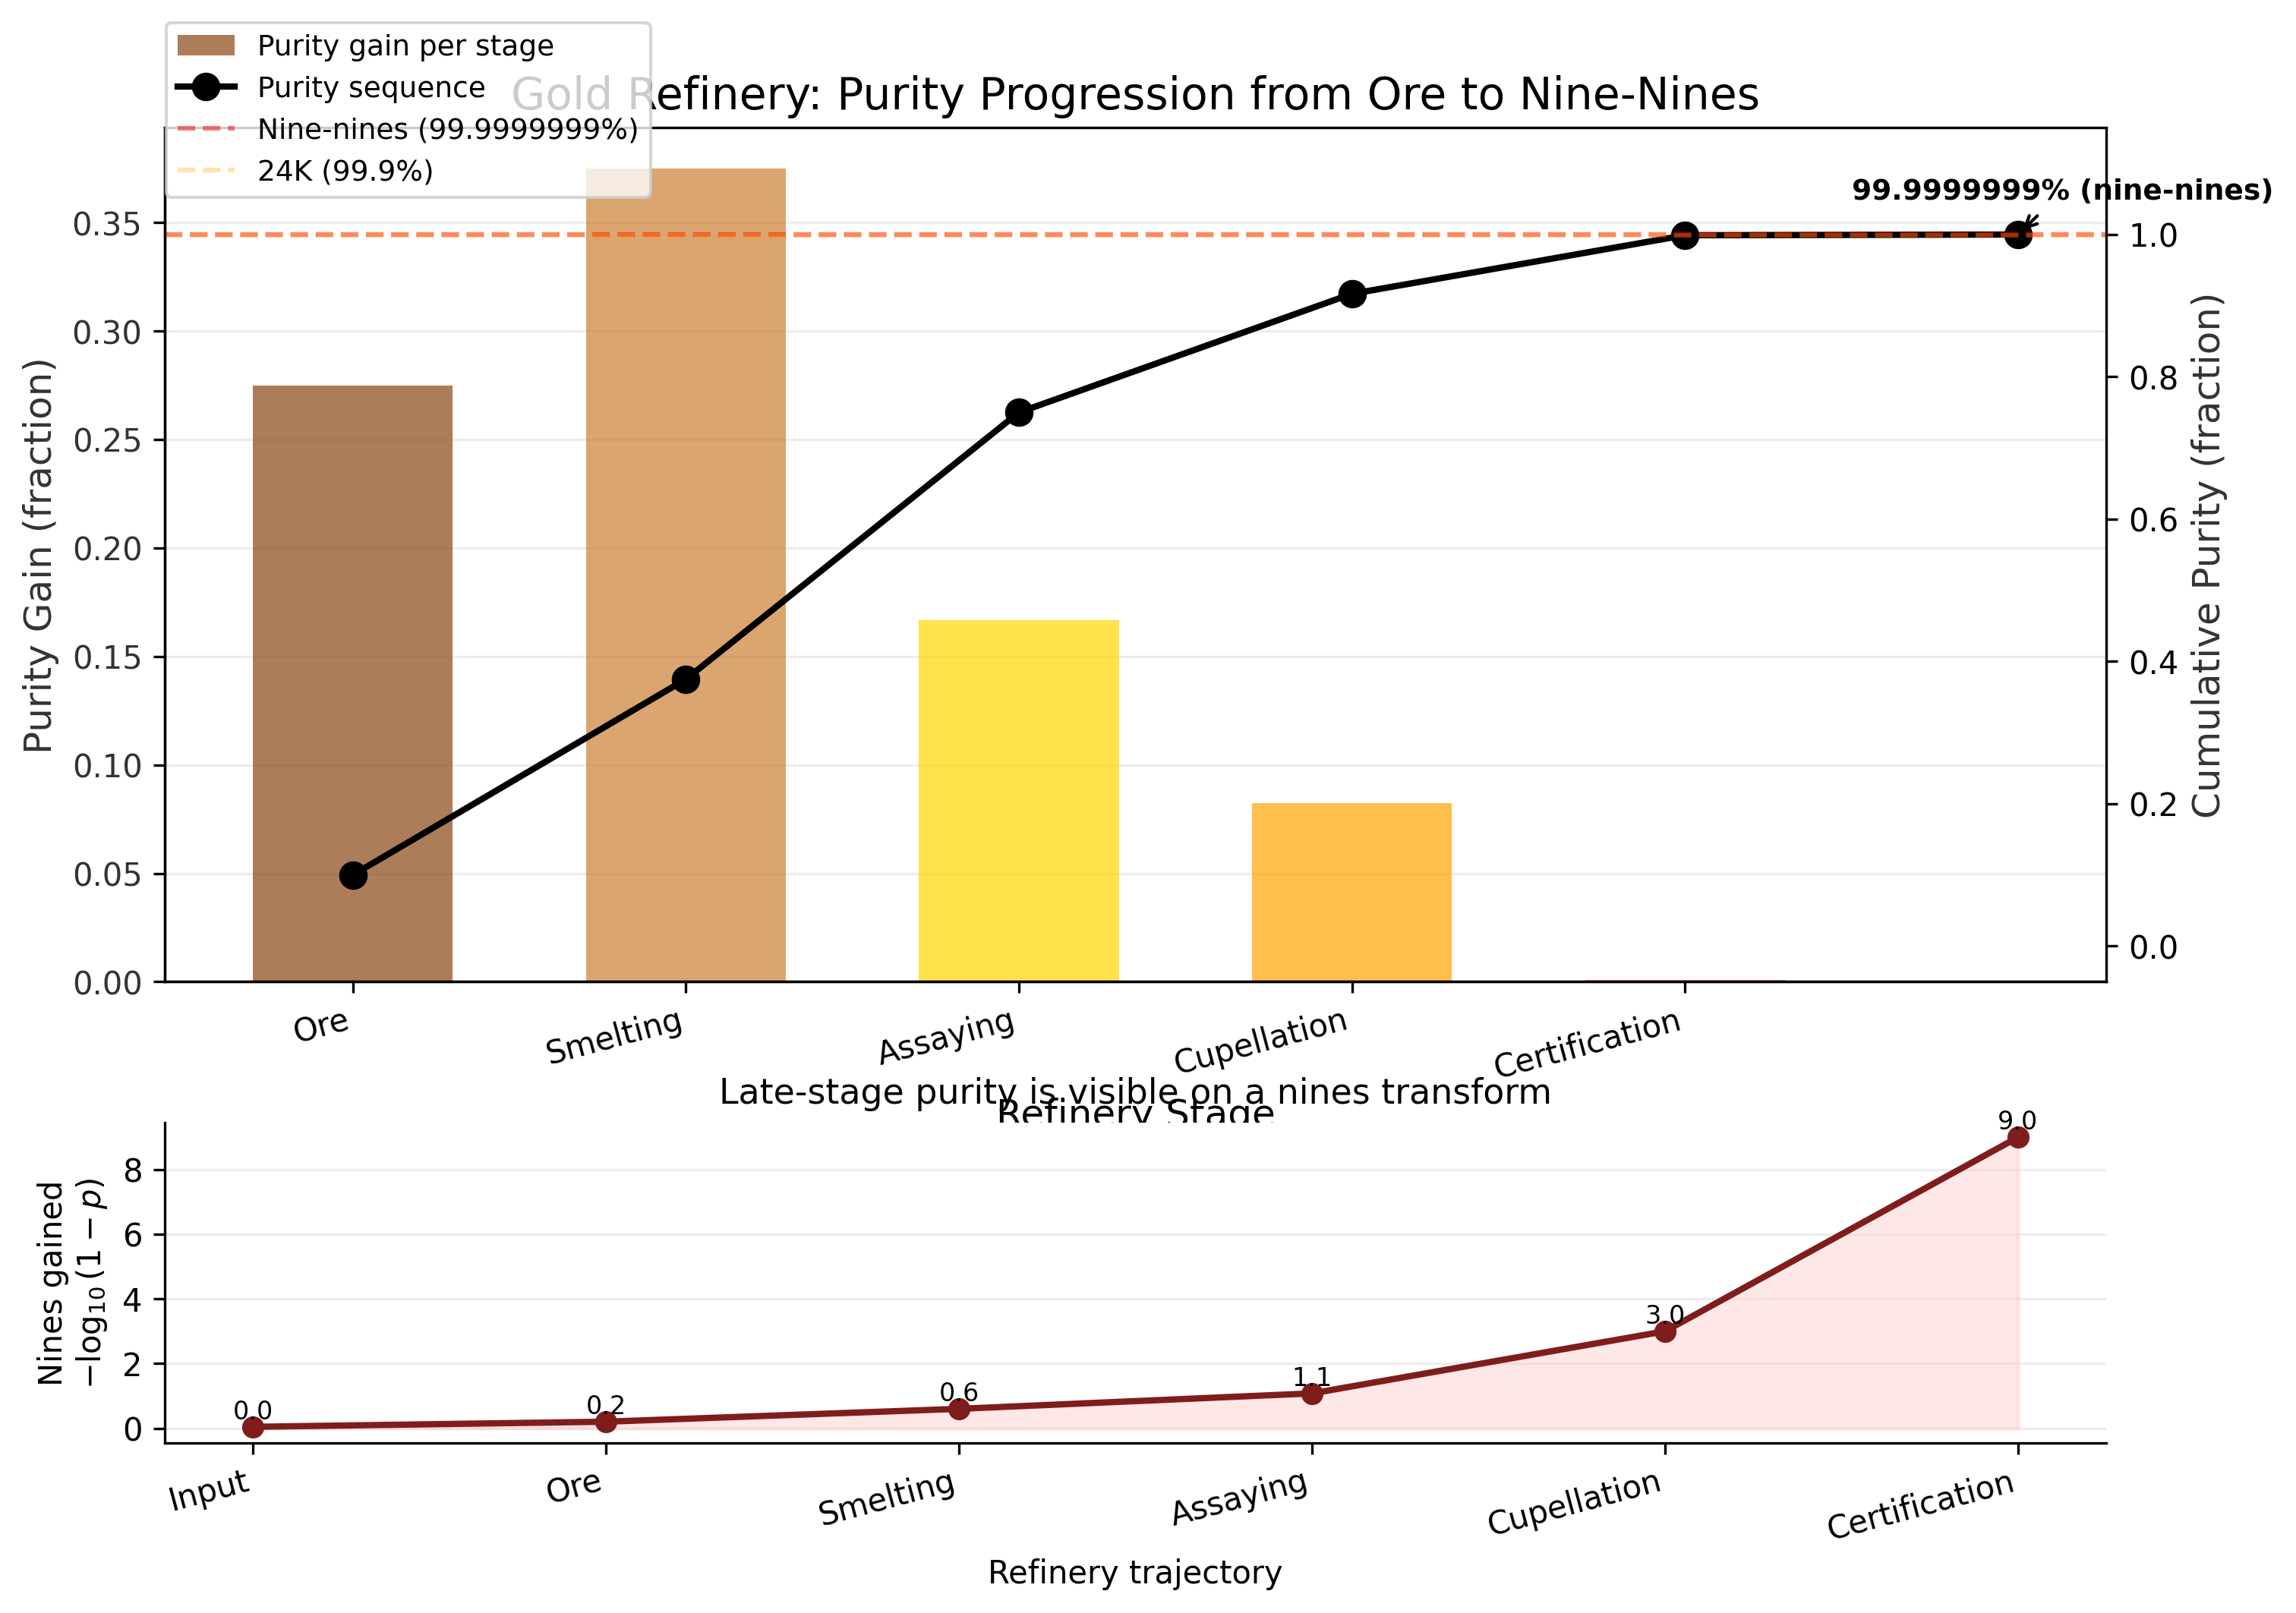
\includegraphics[keepaspectratio,alt={Purity progression across refinery stages}]{../figures/purity_progression.png}}
\caption{Purity progression across refinery
stages}\label{fig:purity_progression}
\end{figure}

{\def\LTcaptype{none} % do not increment counter
\begin{longtable}[]{@{}
  >{\raggedright\arraybackslash}p{(\linewidth - 8\tabcolsep) * \real{0.1750}}
  >{\raggedright\arraybackslash}p{(\linewidth - 8\tabcolsep) * \real{0.1500}}
  >{\raggedright\arraybackslash}p{(\linewidth - 8\tabcolsep) * \real{0.3500}}
  >{\raggedright\arraybackslash}p{(\linewidth - 8\tabcolsep) * \real{0.1750}}
  >{\raggedright\arraybackslash}p{(\linewidth - 8\tabcolsep) * \real{0.1500}}@{}}
\toprule\noalign{}
\begin{minipage}[b]{\linewidth}\raggedright
Stage
\end{minipage} & \begin{minipage}[b]{\linewidth}\raggedright
Name
\end{minipage} & \begin{minipage}[b]{\linewidth}\raggedright
Output purity
\end{minipage} & \begin{minipage}[b]{\linewidth}\raggedright
Karat
\end{minipage} & \begin{minipage}[b]{\linewidth}\raggedright
Gain
\end{minipage} \\
\midrule\noalign{}
\endhead
\bottomrule\noalign{}
\endlastfoot
1 & ore & 37.50\% & 9K & Extract raw gold-bearing ore from the earth \\
2 & smelting & 75.00\% & 18K & Heat ore to separate gold from slag and
dross \\
3 & assaying & 91.67\% & 22K & Test a sample to determine gold content
and impurities \\
4 & cupellation & 99.900\% & 24K & Refine by blowing air through molten
lead-gold alloy \\
5 & certification & 99.9999999\% (nine-nines) & 24K (nine-nines
certified) & Certify purity grade and stamp hallmark \\
\end{longtable}
}

\subsection{Karat grading scale}\label{karat-grading-scale}

\begin{figure}
\centering
\pandocbounded{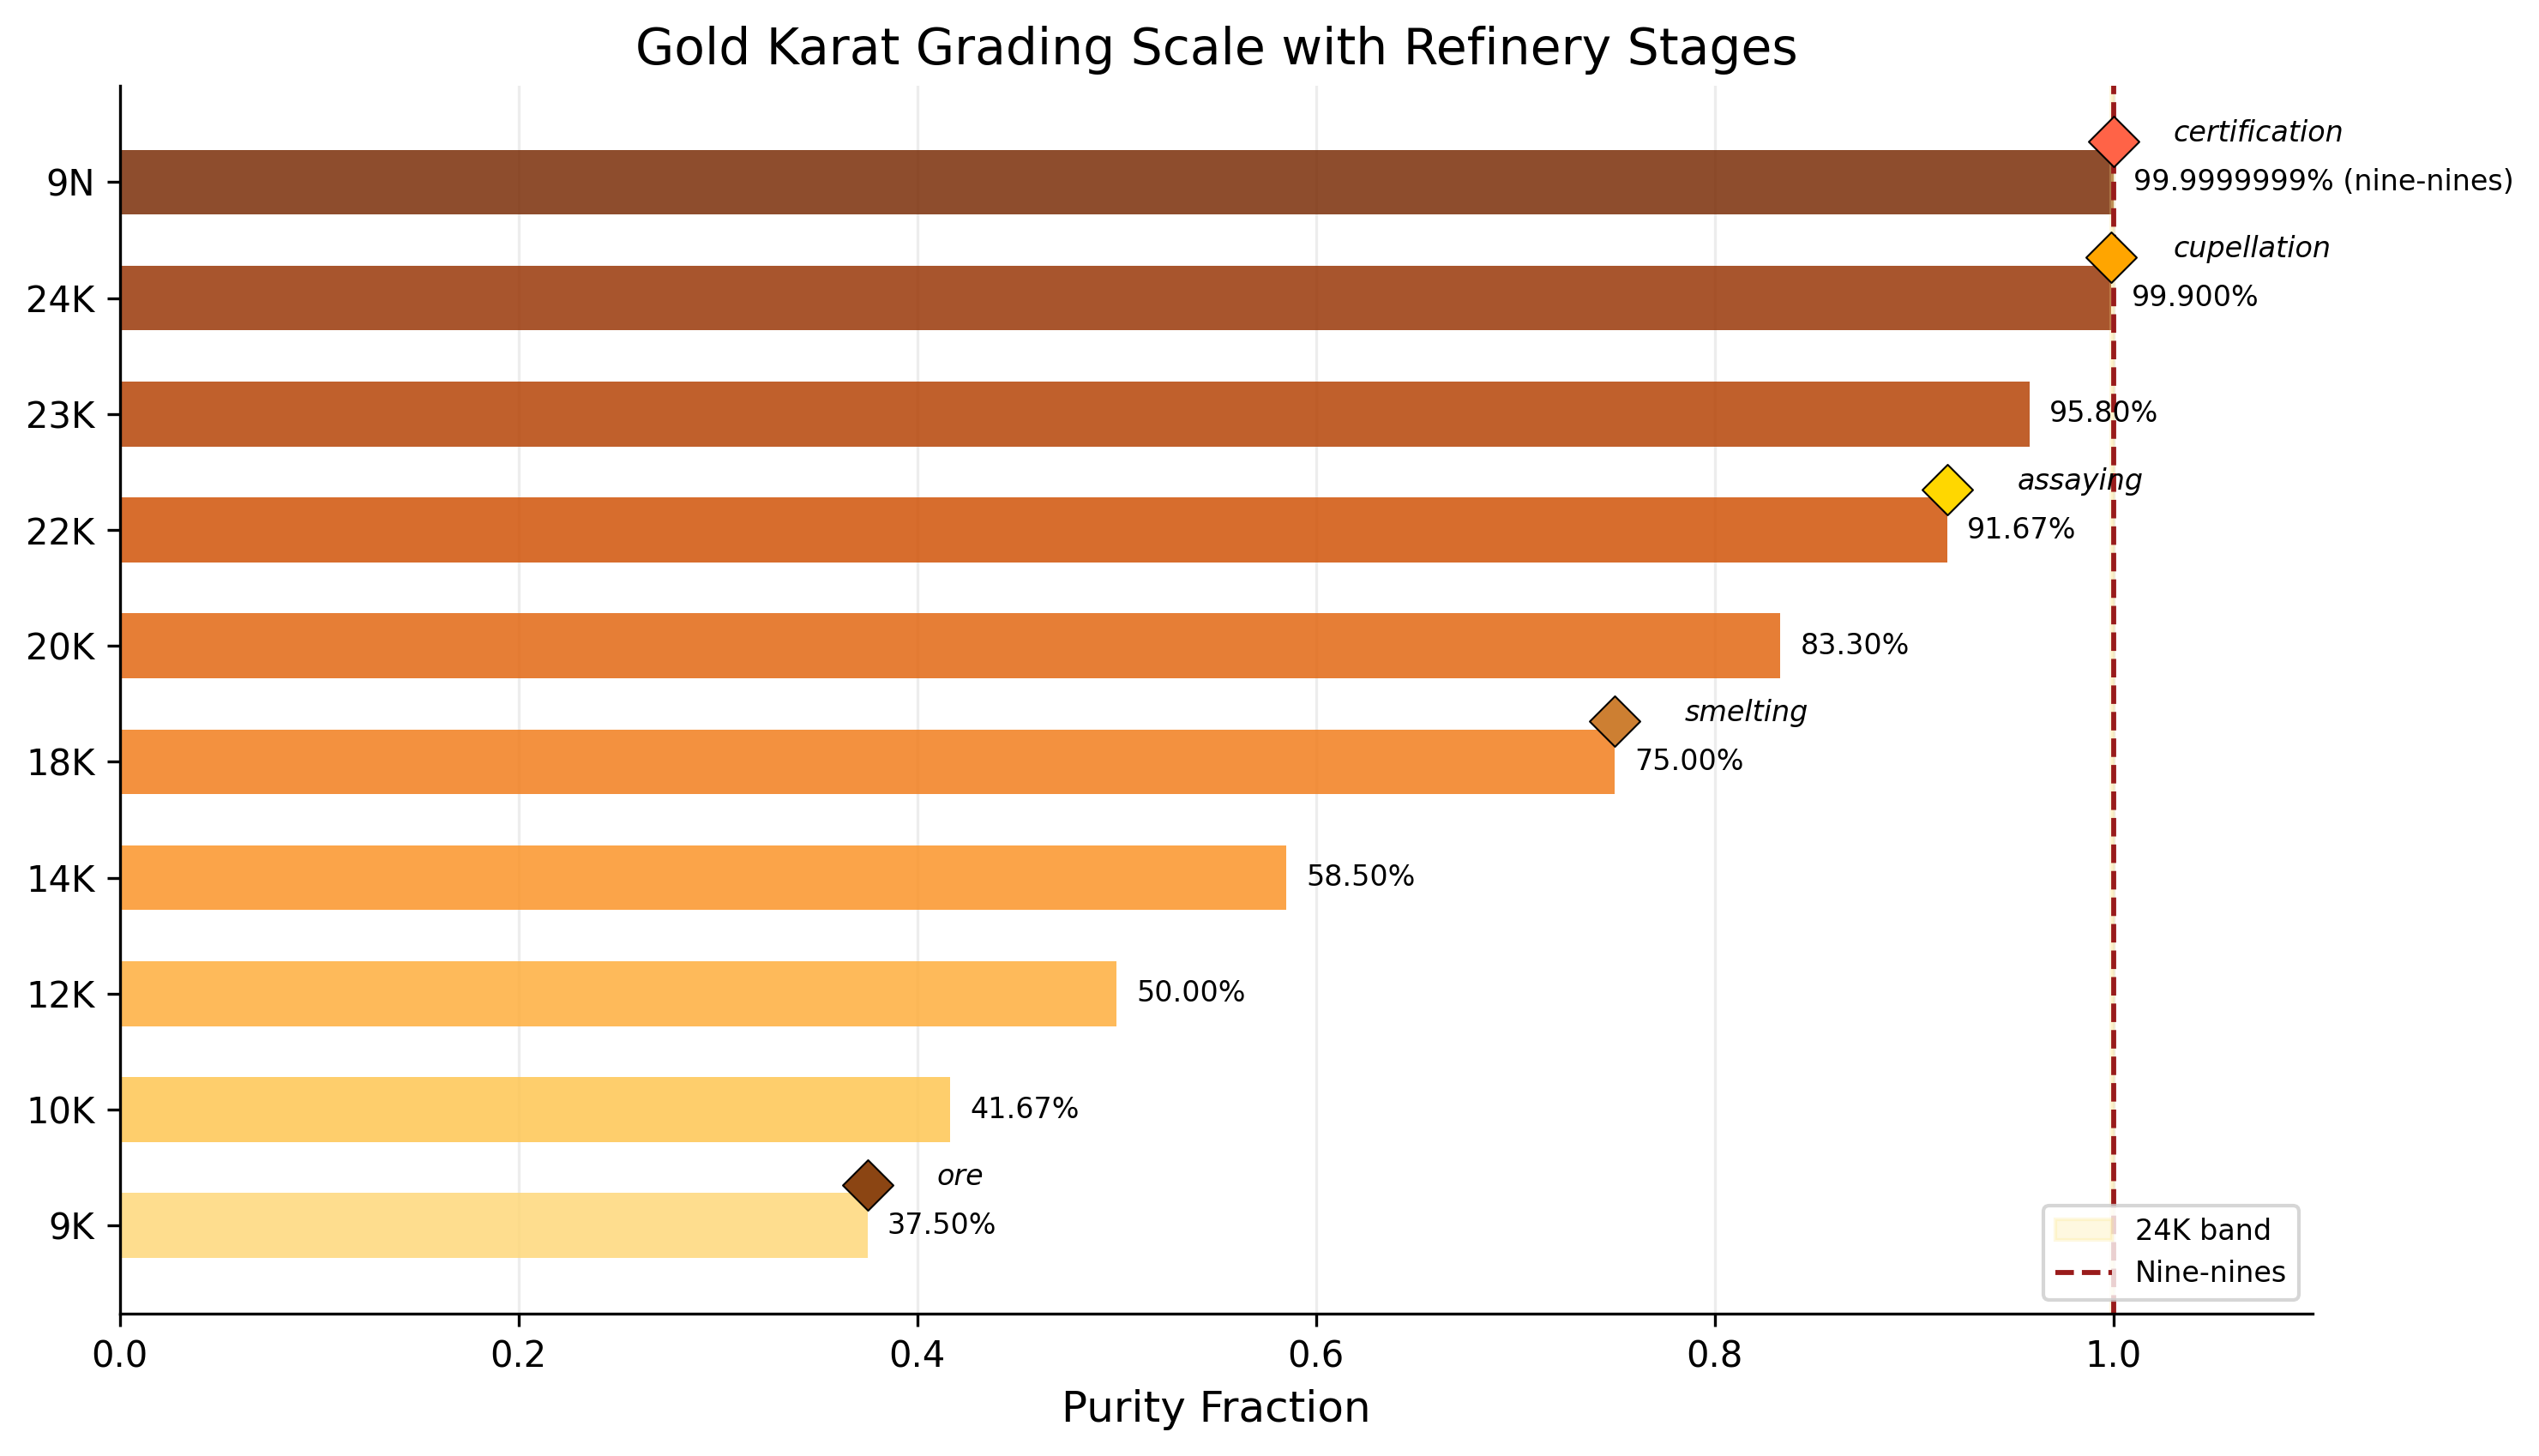
\includegraphics[keepaspectratio,alt={Gold karat grading scale with refinery stage markers}]{../figures/karat_grading.png}}
\caption{Gold karat grading scale with refinery stage
markers}\label{fig:karat_grading}
\end{figure}

\subsection{Final certification}\label{final-certification}

\begin{itemize}
\tightlist
\item
  \textbf{Final purity:} 99.9999999\% (nine-nines)
\item
  \textbf{Final karat:} 24K (nine-nines certified)
\item
  \textbf{Total purity gain:} 90.00\%
\item
  \textbf{Nine-nines certified:} Yes
\item
  \textbf{Nines count:} 9
\end{itemize}

\subsection{Token plan summary}\label{token-plan-summary}

The mega-madlib engine generated 24 tokens from seed 431 across 8
lexicon categories.

\begin{figure}
\centering
\pandocbounded{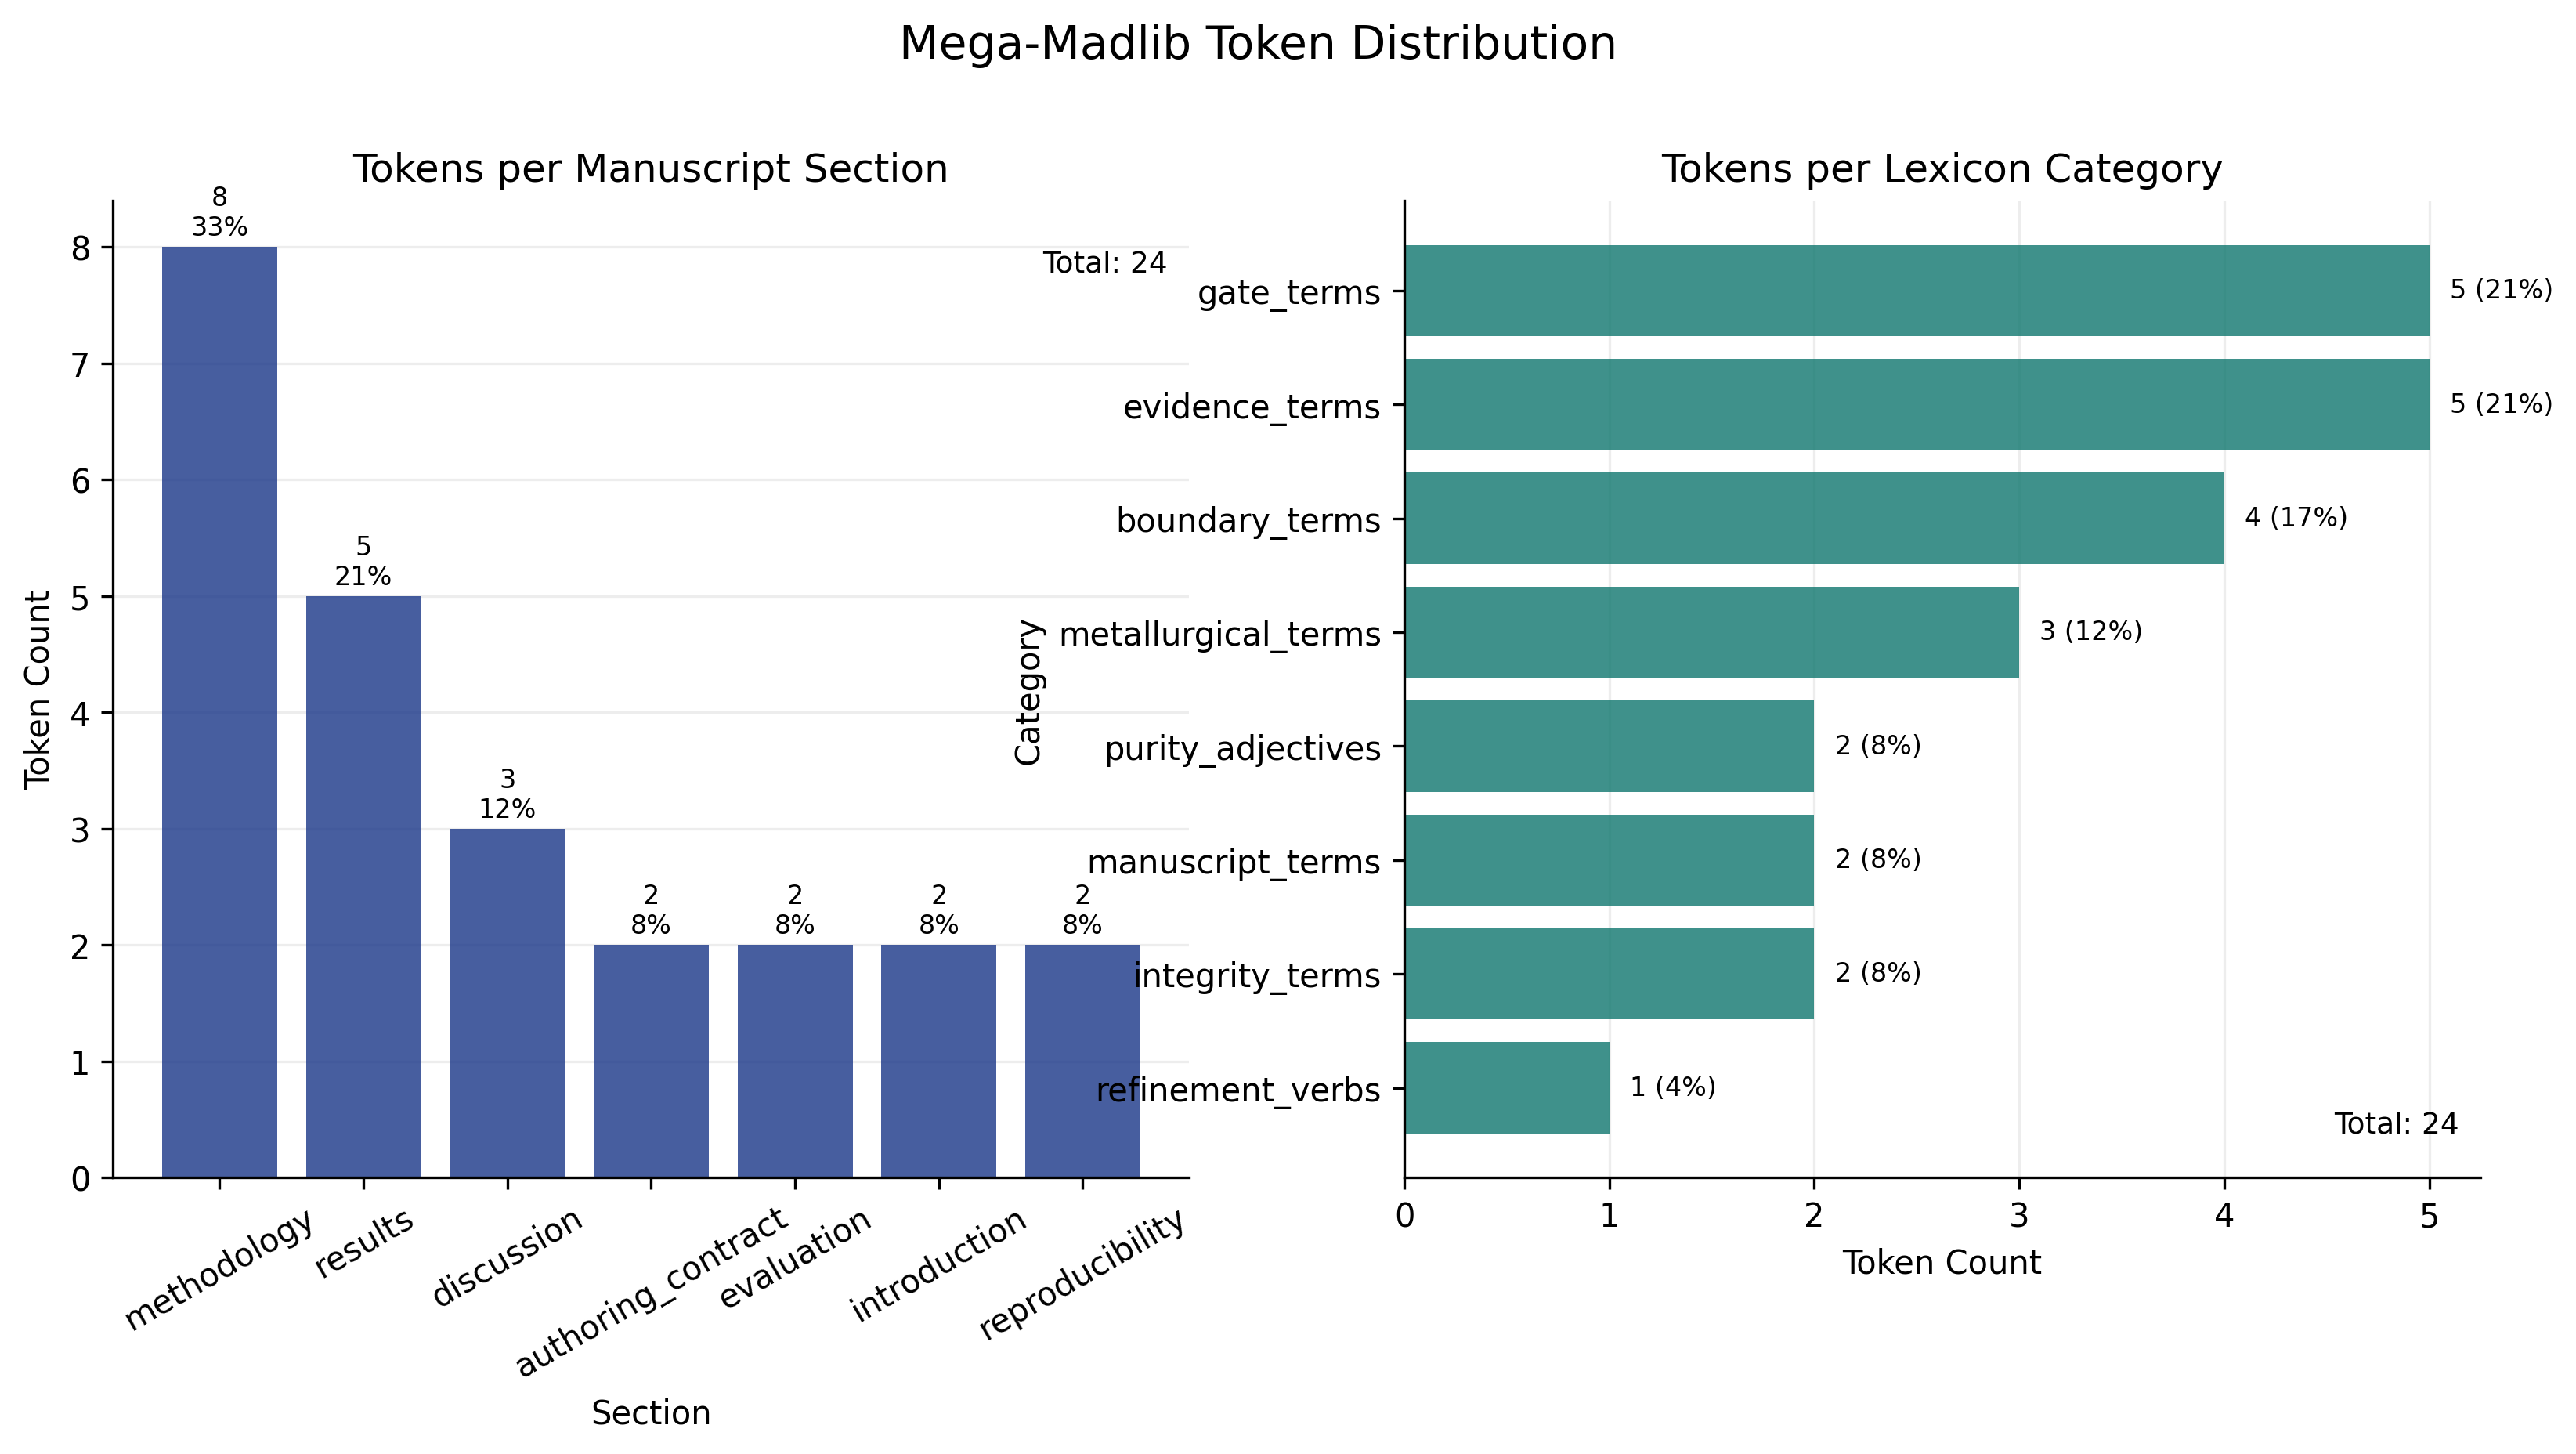
\includegraphics[keepaspectratio,alt={Mega-madlib token distribution}]{../figures/token_density.png}}
\caption{Mega-madlib token distribution}\label{fig:token_density}
\end{figure}

\subsubsection{Category distribution}\label{category-distribution}

{\def\LTcaptype{none} % do not increment counter
\begin{longtable}[]{@{}ll@{}}
\toprule\noalign{}
Category & Count \\
\midrule\noalign{}
\endhead
\bottomrule\noalign{}
\endlastfoot
boundary\_terms & 4 \\
evidence\_terms & 5 \\
gate\_terms & 5 \\
integrity\_terms & 2 \\
manuscript\_terms & 2 \\
metallurgical\_terms & 3 \\
purity\_adjectives & 2 \\
refinement\_verbs & 1 \\
\end{longtable}
}

\subsubsection{Section distribution}\label{section-distribution}

{\def\LTcaptype{none} % do not increment counter
\begin{longtable}[]{@{}ll@{}}
\toprule\noalign{}
Section & Token count \\
\midrule\noalign{}
\endhead
\bottomrule\noalign{}
\endlastfoot
authoring\_contract & 2 \\
discussion & 3 \\
evaluation & 2 \\
introduction & 2 \\
methodology & 8 \\
reproducibility & 2 \\
results & 5 \\
\end{longtable}
}

\subsubsection{Provenance trace}\label{provenance-trace}

{\def\LTcaptype{none} % do not increment counter
\begin{longtable}[]{@{}
  >{\raggedright\arraybackslash}p{(\linewidth - 8\tabcolsep) * \real{0.2273}}
  >{\raggedright\arraybackslash}p{(\linewidth - 8\tabcolsep) * \real{0.2273}}
  >{\raggedright\arraybackslash}p{(\linewidth - 8\tabcolsep) * \real{0.1591}}
  >{\raggedright\arraybackslash}p{(\linewidth - 8\tabcolsep) * \real{0.2045}}
  >{\raggedright\arraybackslash}p{(\linewidth - 8\tabcolsep) * \real{0.1818}}@{}}
\toprule\noalign{}
\begin{minipage}[b]{\linewidth}\raggedright
Variable
\end{minipage} & \begin{minipage}[b]{\linewidth}\raggedright
Category
\end{minipage} & \begin{minipage}[b]{\linewidth}\raggedright
Value
\end{minipage} & \begin{minipage}[b]{\linewidth}\raggedright
Section
\end{minipage} & \begin{minipage}[b]{\linewidth}\raggedright
Source
\end{minipage} \\
\midrule\noalign{}
\endhead
\bottomrule\noalign{}
\endlastfoot
AUTHORING\_BOUNDARY\_TERM\_1 & boundary\_terms & analogy boundary &
authoring\_contract &
manuscript/config.yaml\#gold\_refinement.lexicon.boundary\_terms{[}1{]} \\
AUTHORING\_BOUNDARY\_TERM\_2 & boundary\_terms & non-claim &
authoring\_contract &
manuscript/config.yaml\#gold\_refinement.lexicon.boundary\_terms{[}4{]} \\
DISCUSSION\_BOUNDARY\_TERM\_1 & boundary\_terms & fork obligation &
discussion &
manuscript/config.yaml\#gold\_refinement.lexicon.boundary\_terms{[}2{]} \\
DISCUSSION\_BOUNDARY\_TERM\_2 & boundary\_terms & domain validator &
discussion &
manuscript/config.yaml\#gold\_refinement.lexicon.boundary\_terms{[}3{]} \\
DISCUSSION\_REFINEMENT\_VERB & refinement\_verbs & smelting & discussion
&
manuscript/config.yaml\#gold\_refinement.lexicon.refinement\_verbs{[}3{]} \\
EVALUATION\_GATE\_TERM\_1 & gate\_terms & prerender & evaluation &
manuscript/config.yaml\#gold\_refinement.lexicon.gate\_terms{[}0{]} \\
EVALUATION\_GATE\_TERM\_2 & gate\_terms & citation validation &
evaluation &
manuscript/config.yaml\#gold\_refinement.lexicon.gate\_terms{[}3{]} \\
INTRO\_INTEGRITY\_TERM\_1 & integrity\_terms & source tier &
introduction &
manuscript/config.yaml\#gold\_refinement.lexicon.integrity\_terms{[}1{]} \\
INTRO\_INTEGRITY\_TERM\_2 & integrity\_terms & evidence spine &
introduction &
manuscript/config.yaml\#gold\_refinement.lexicon.integrity\_terms{[}0{]} \\
METHOD\_GATE\_TERM\_1 & gate\_terms & evidence validation & methodology
& manuscript/config.yaml\#gold\_refinement.lexicon.gate\_terms{[}1{]} \\
METHOD\_GATE\_TERM\_2 & gate\_terms & figure registry check &
methodology &
manuscript/config.yaml\#gold\_refinement.lexicon.gate\_terms{[}2{]} \\
METHOD\_GATE\_TERM\_3 & gate\_terms & citation validation & methodology
& manuscript/config.yaml\#gold\_refinement.lexicon.gate\_terms{[}3{]} \\
METHOD\_MANUSCRIPT\_TERM\_1 & manuscript\_terms & evidence & methodology
&
manuscript/config.yaml\#gold\_refinement.lexicon.manuscript\_terms{[}4{]} \\
METHOD\_MANUSCRIPT\_TERM\_2 & manuscript\_terms & evidence & methodology
&
manuscript/config.yaml\#gold\_refinement.lexicon.manuscript\_terms{[}4{]} \\
METHOD\_METAL\_TERM\_1 & metallurgical\_terms & assaying & methodology &
manuscript/config.yaml\#gold\_refinement.lexicon.metallurgical\_terms{[}1{]} \\
METHOD\_METAL\_TERM\_2 & metallurgical\_terms & parting & methodology &
manuscript/config.yaml\#gold\_refinement.lexicon.metallurgical\_terms{[}3{]} \\
METHOD\_METAL\_TERM\_3 & metallurgical\_terms & smelting & methodology &
manuscript/config.yaml\#gold\_refinement.lexicon.metallurgical\_terms{[}2{]} \\
REPRO\_EVIDENCE\_TERM\_1 & evidence\_terms & fact registry &
reproducibility &
manuscript/config.yaml\#gold\_refinement.lexicon.evidence\_terms{[}0{]} \\
REPRO\_EVIDENCE\_TERM\_2 & evidence\_terms & figure registry &
reproducibility &
manuscript/config.yaml\#gold\_refinement.lexicon.evidence\_terms{[}3{]} \\
RESULTS\_EVIDENCE\_TERM\_1 & evidence\_terms & artifact manifest &
results &
manuscript/config.yaml\#gold\_refinement.lexicon.evidence\_terms{[}1{]} \\
RESULTS\_EVIDENCE\_TERM\_2 & evidence\_terms & figure registry & results
&
manuscript/config.yaml\#gold\_refinement.lexicon.evidence\_terms{[}3{]} \\
RESULTS\_EVIDENCE\_TERM\_3 & evidence\_terms & token provenance &
results &
manuscript/config.yaml\#gold\_refinement.lexicon.evidence\_terms{[}4{]} \\
RESULTS\_PURITY\_ADJ\_1 & purity\_adjectives & unrefined & results &
manuscript/config.yaml\#gold\_refinement.lexicon.purity\_adjectives{[}0{]} \\
RESULTS\_PURITY\_ADJ\_2 & purity\_adjectives & purified & results &
manuscript/config.yaml\#gold\_refinement.lexicon.purity\_adjectives{[}1{]} \\
\end{longtable}
}

Selected purity adjectives for this section: unrefined, purified.
Selected evidence terms: artifact manifest, figure registry, token
provenance.

\subsection{Provenance flow}\label{provenance-flow}

\begin{figure}
\centering
\pandocbounded{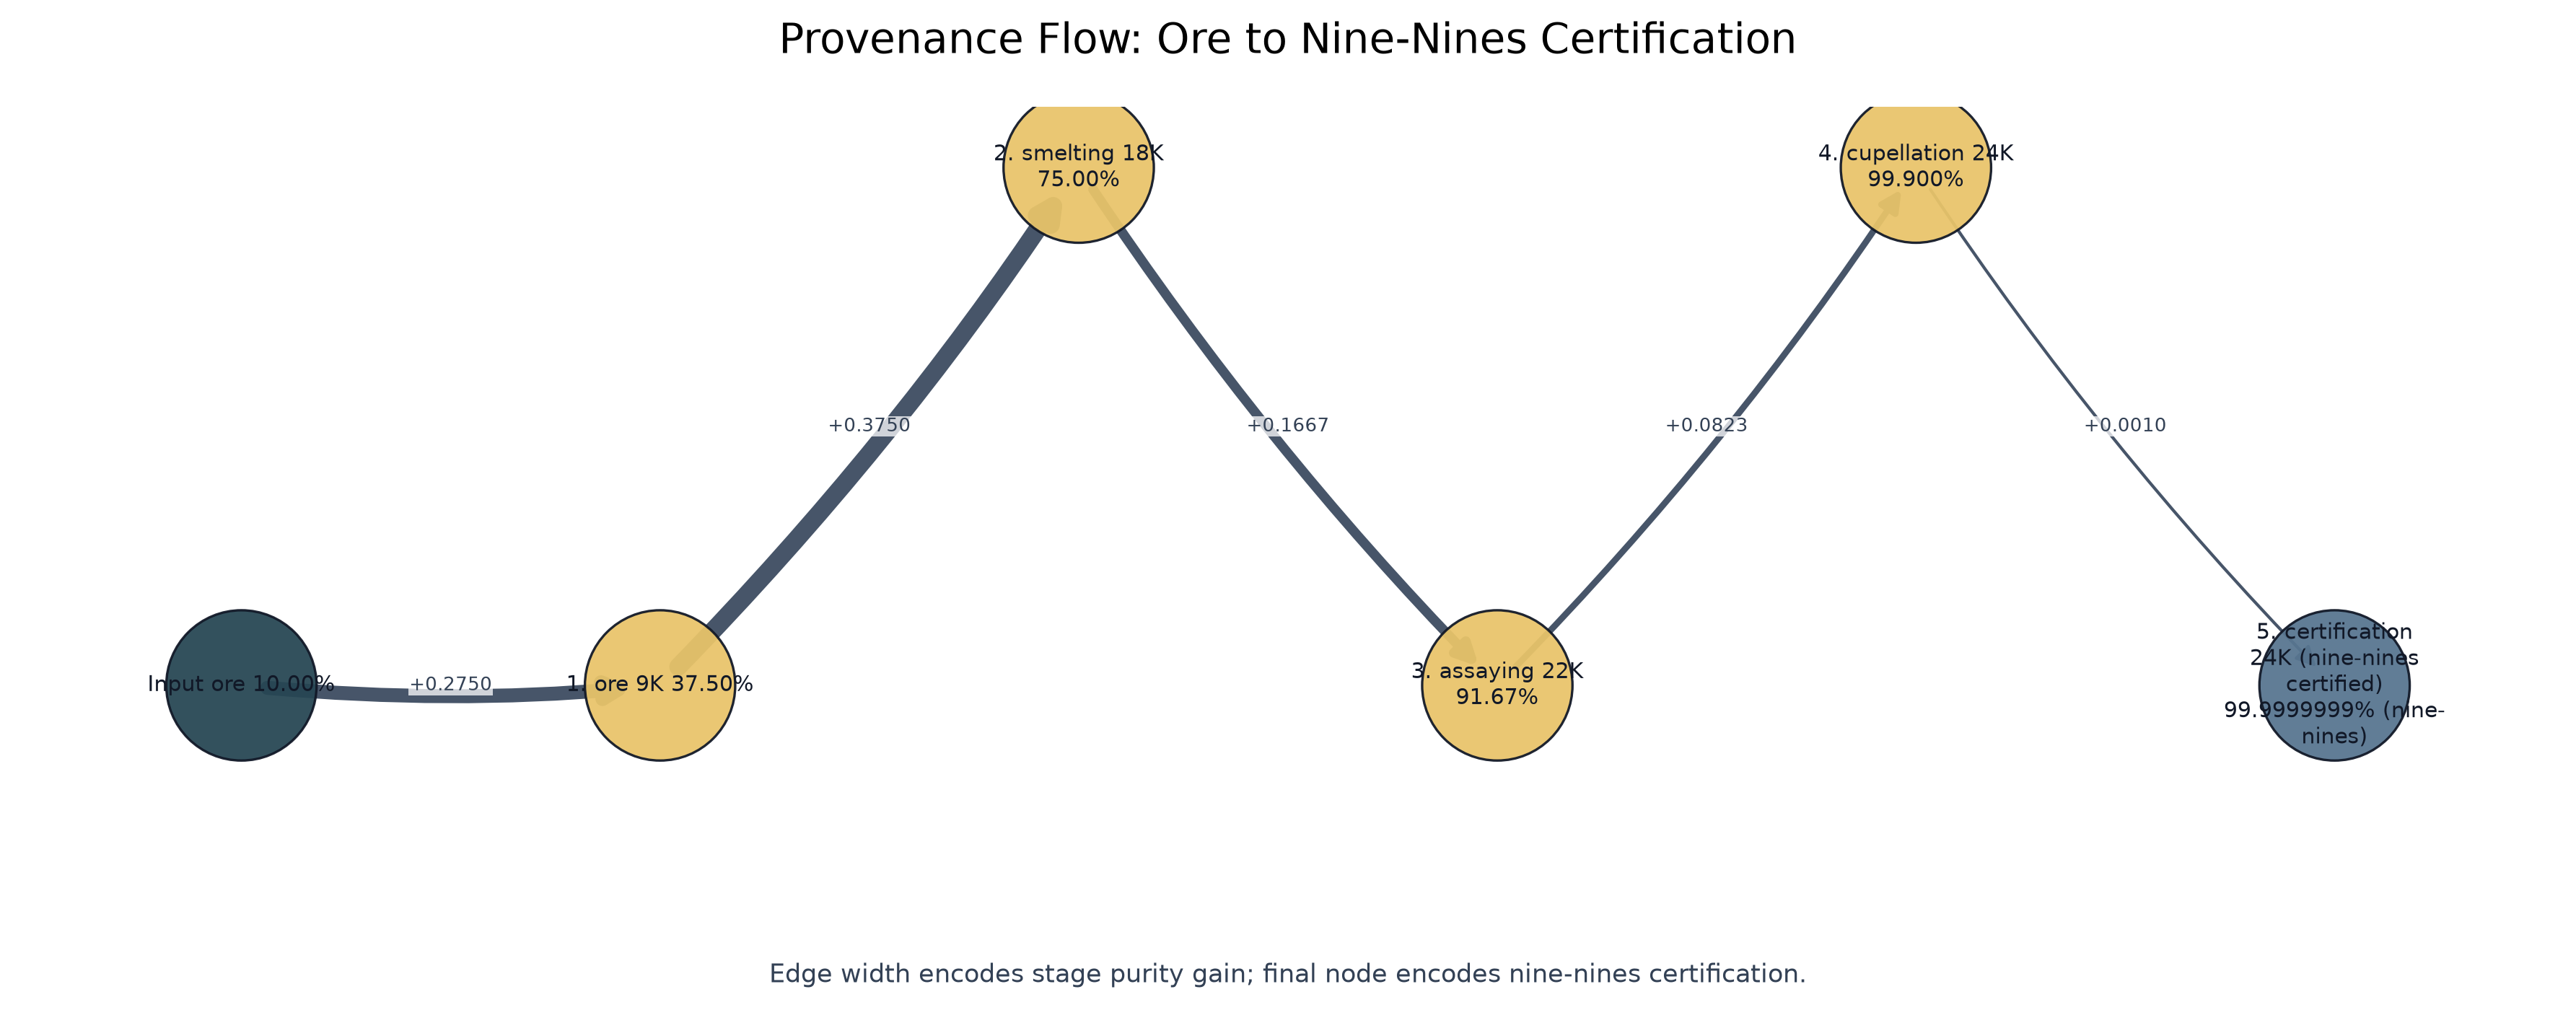
\includegraphics[keepaspectratio,alt={Provenance flow diagram}]{../figures/provenance_sankey.png}}
\caption{Provenance flow diagram}\label{fig:provenance_sankey}
\end{figure}

\subsection{Purity vs claim support}\label{purity-vs-claim-support}

\begin{figure}
\centering
\pandocbounded{
\includegraphics[keepaspectratio,alt={Purity vs claim support}]{../figures/purity_claim_scatter.png}}
\caption{Purity vs claim support}\label{fig:purity_claim_scatter}
\end{figure}

\subsection{Token selection
sensitivity}\label{token-selection-sensitivity}

\begin{figure}
\centering
\pandocbounded{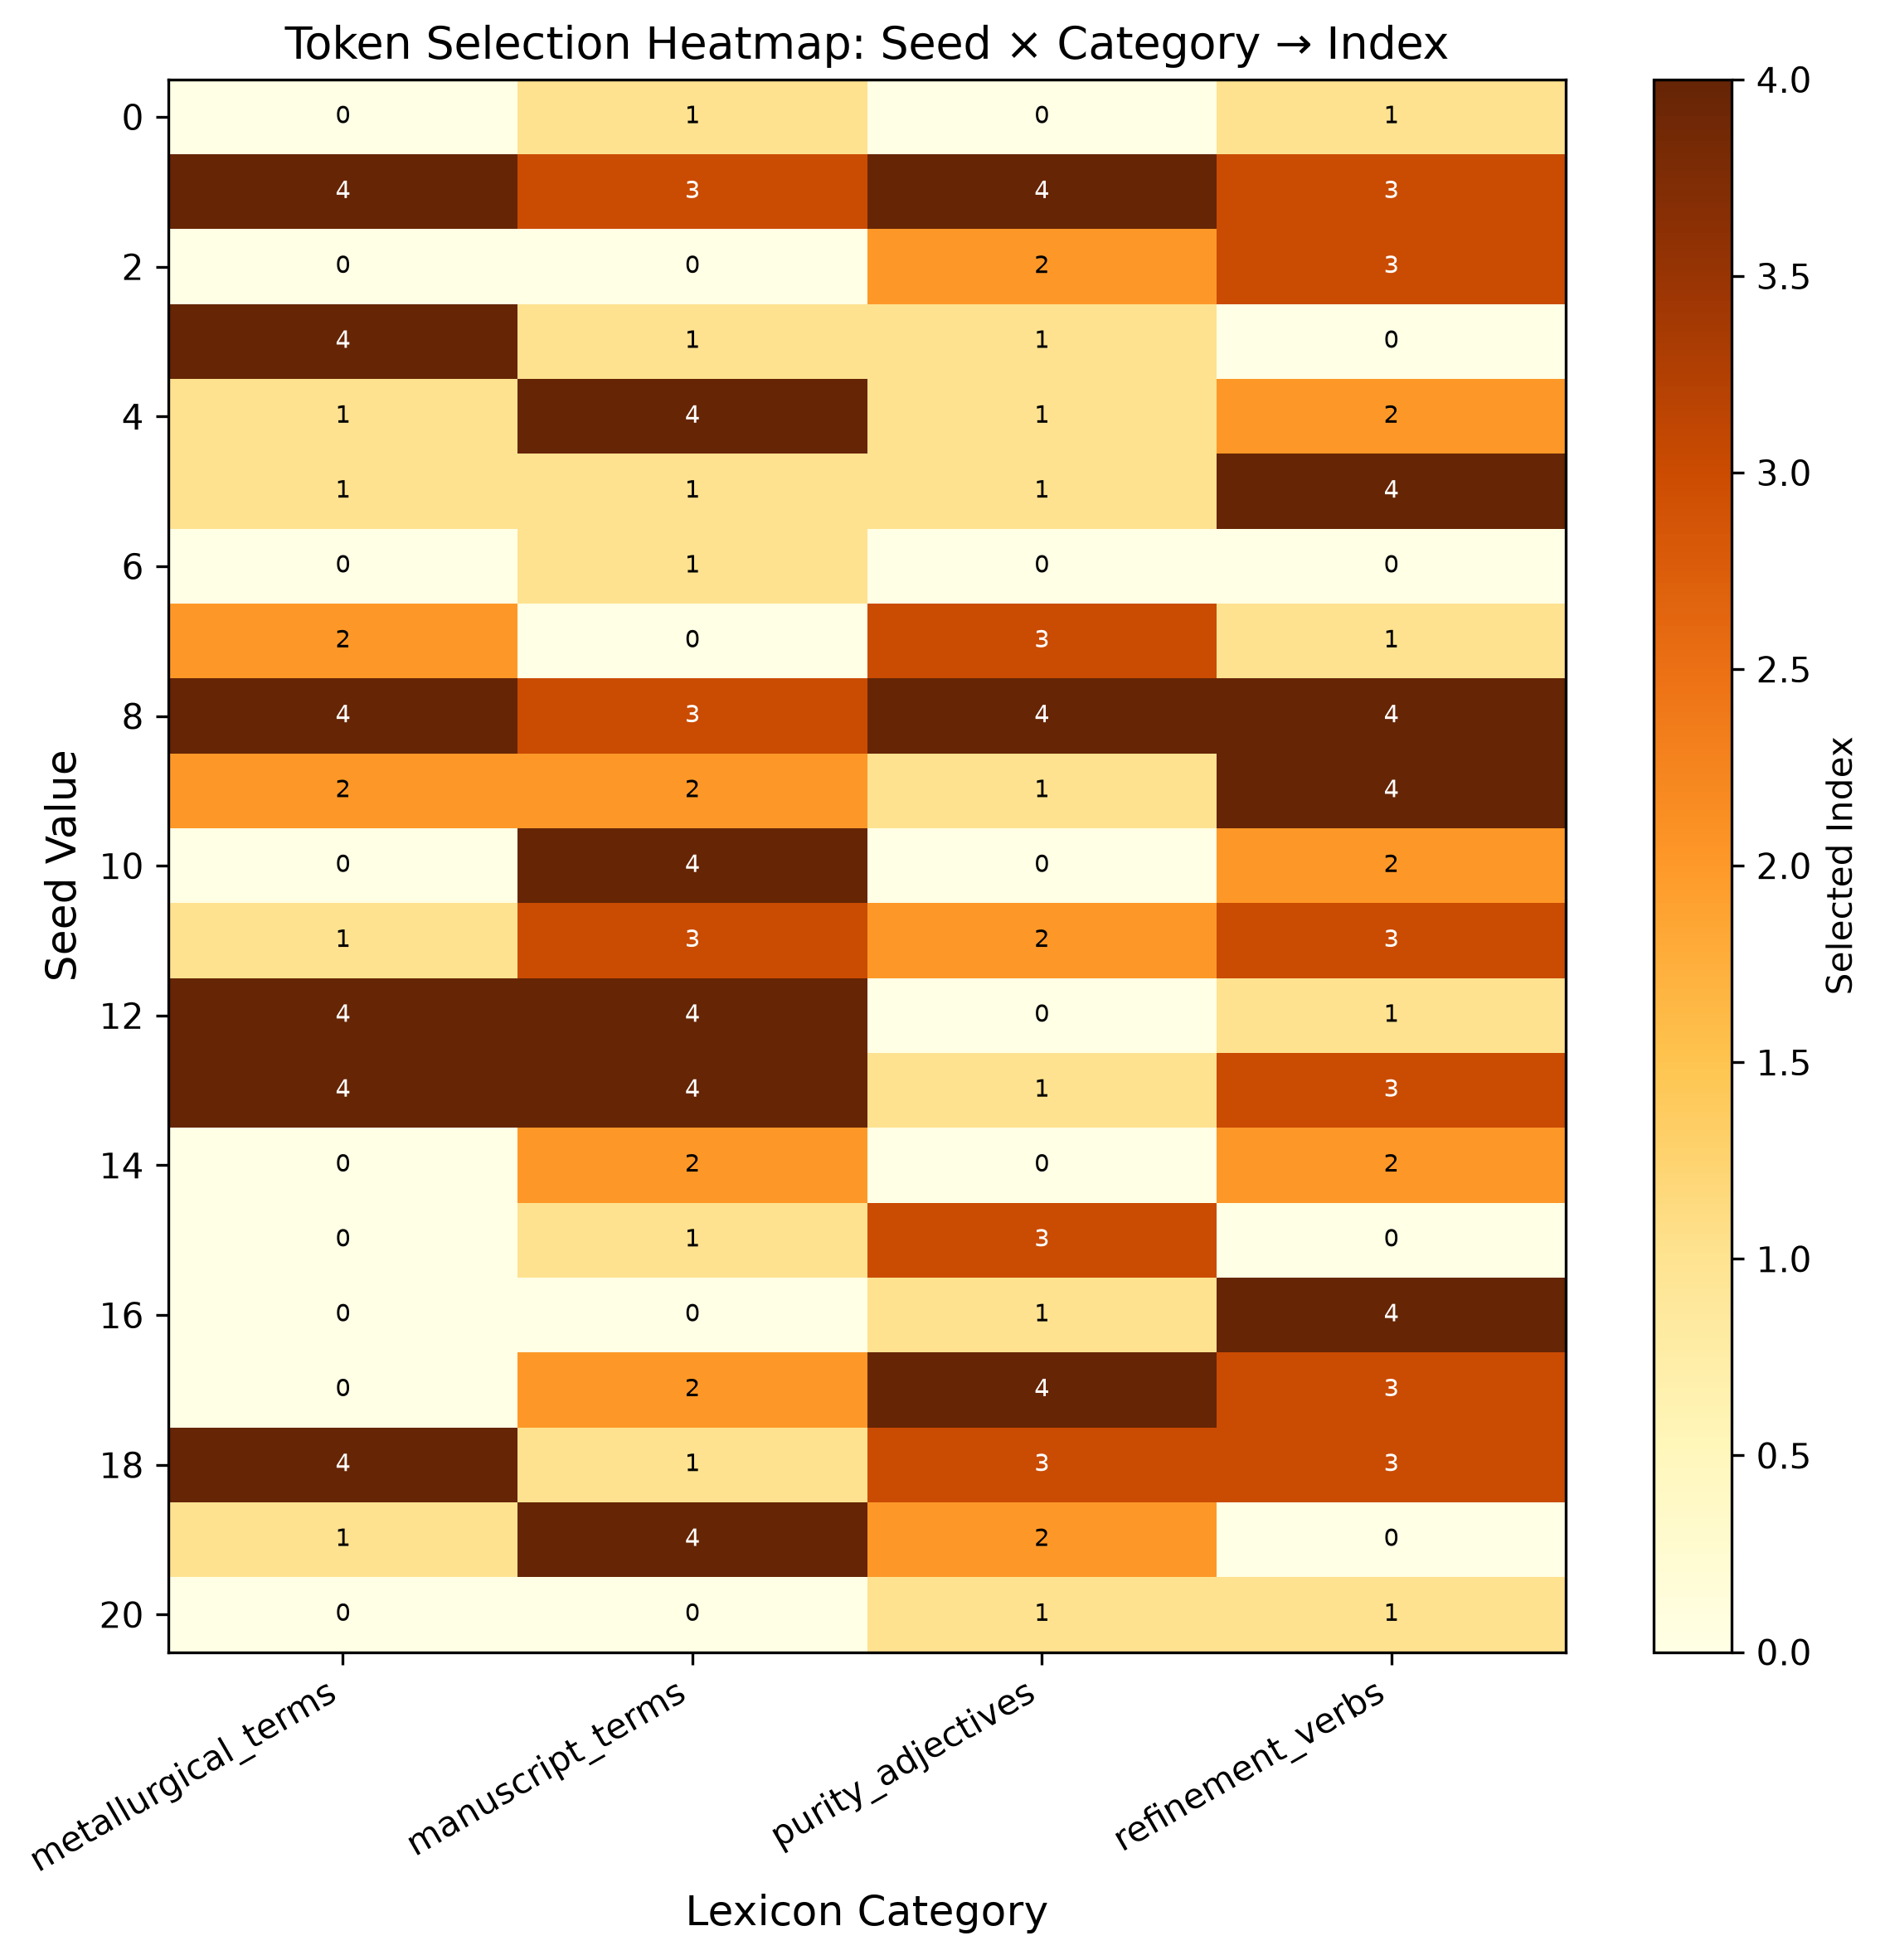
\includegraphics[keepaspectratio,alt={Token selection heatmap}]{../figures/token_heatmap.png}}
\caption{Token selection heatmap}\label{fig:token_heatmap}
\end{figure}

\subsection{Integrity gate matrix}\label{integrity-gate-matrix}

The integrity gate matrix in fig.~\ref{fig:integrity_gate_matrix} makes
the validation story visible: audit rules are not prose promises unless
they connect to tests, manuscript surfaces, and generated artifacts.

\begin{figure}
\centering
\pandocbounded{
\includegraphics[keepaspectratio,alt={Integrity-gate matrix}]{../figures/integrity_gate_matrix.png}}
\caption{Integrity-gate matrix}\label{fig:integrity_gate_matrix}
\end{figure}

\subsection{Formalism traceability}\label{formalism-traceability}

The formalism traceability view in fig.~\ref{fig:formalism_traceability}
links each equation-backed formalism to the source surface that owns it.
This is the visual counterpart to tbl.~\ref{tbl:formalism_registry}.

\begin{figure}
\centering
\pandocbounded{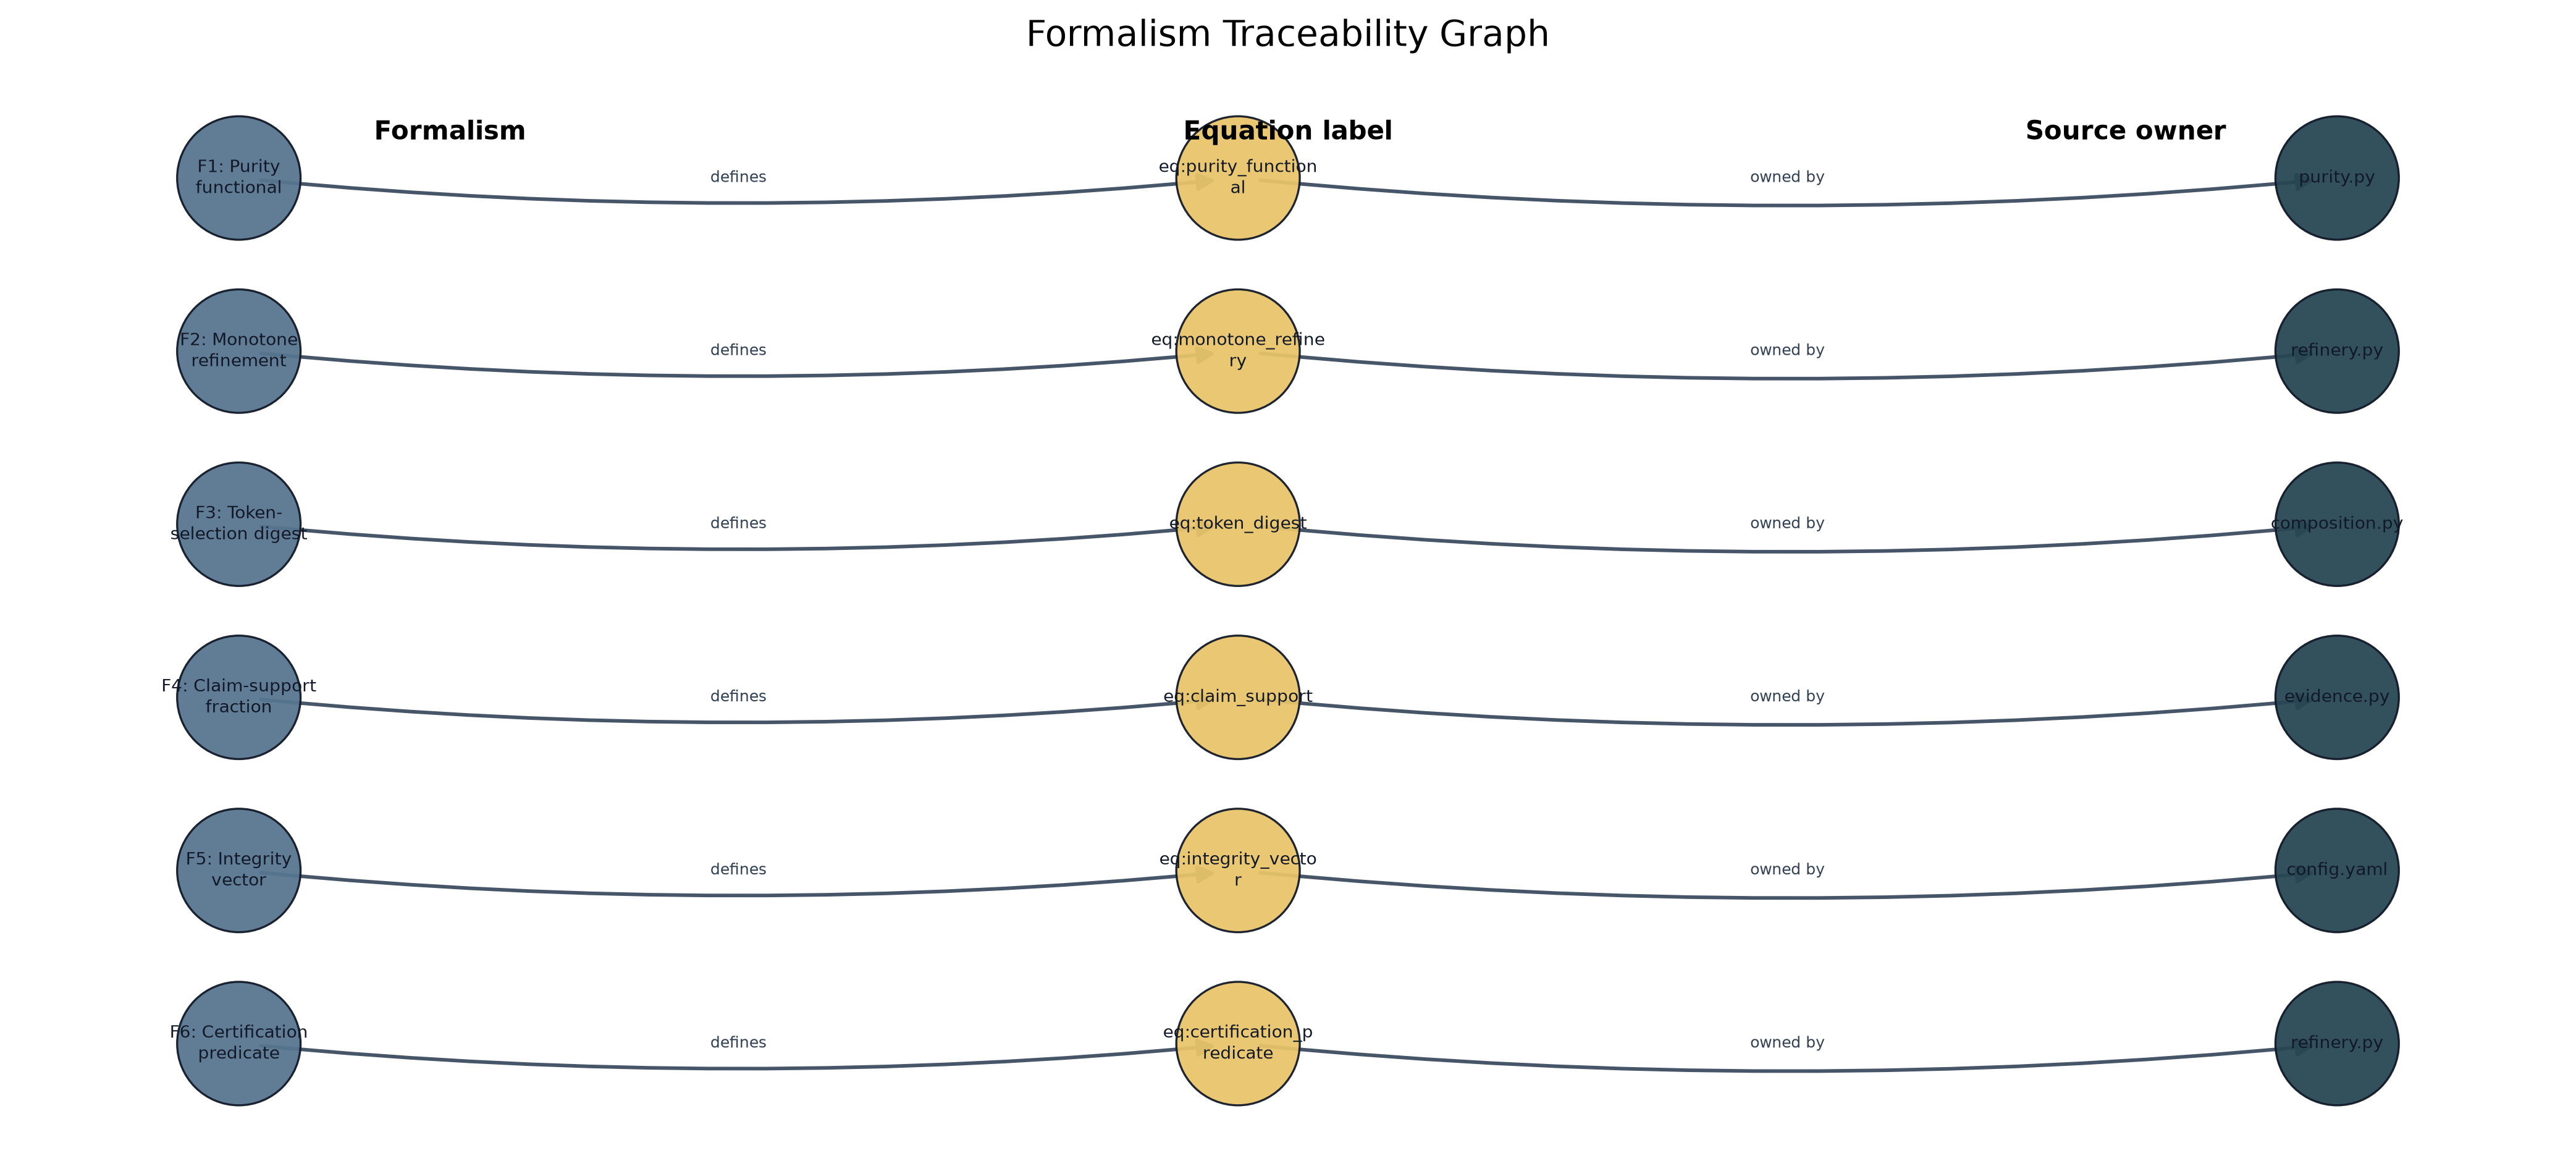
\includegraphics[keepaspectratio,alt={Formalism traceability}]{../figures/formalism_traceability.png}}
\caption{Formalism traceability}\label{fig:formalism_traceability}
\end{figure}

\subsection{Implementation circuit}\label{implementation-circuit-1}

The implementation circuit in fig.~\ref{fig:implementation_circuit}
shows how the concept is executed rather than merely described.
Configuration feeds code; code emits variables, figures, and reports;
manuscript hydration consumes those artifacts; validators feed errors
back to source ownership. The figure is intentionally circular because
the artifact is not complete after prose generation. It is complete only
after the validation return path has no blocking evidence, citation,
reference, or render failures.

\begin{figure}
\centering
\pandocbounded{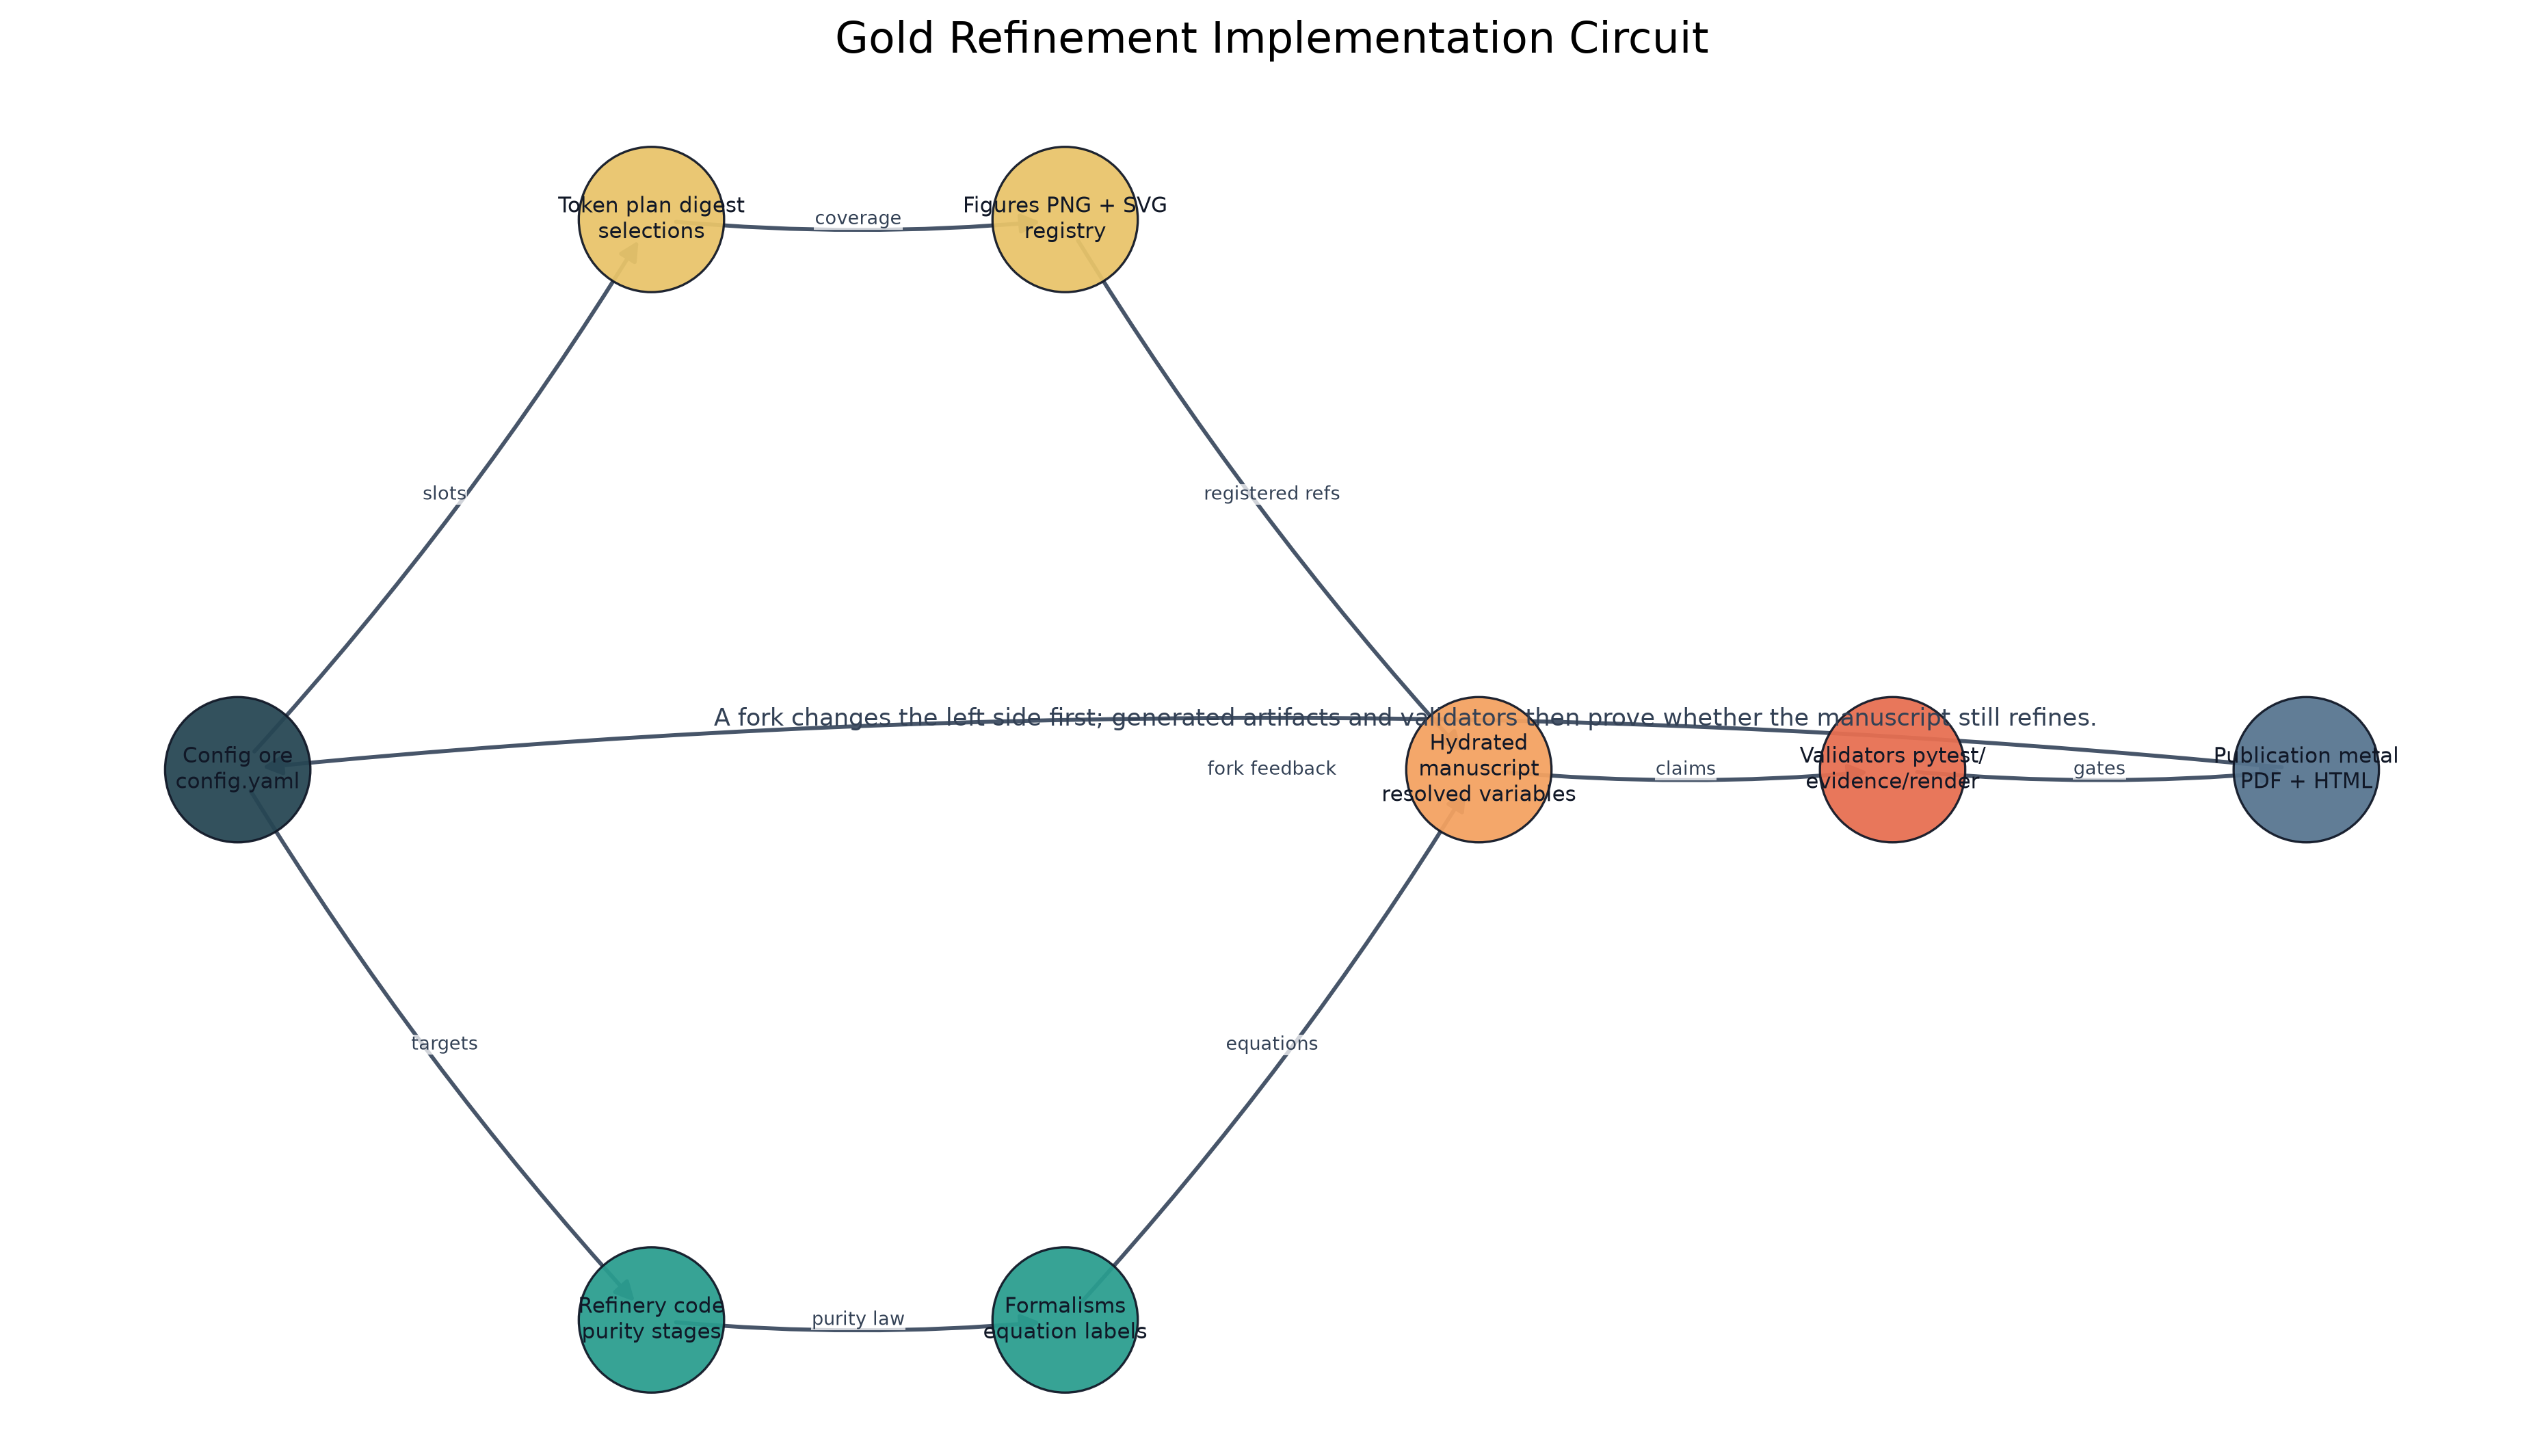
\includegraphics[keepaspectratio,alt={Gold-refinement implementation circuit}]{../figures/implementation_circuit.png}}
\caption{Gold-refinement implementation
circuit}\label{fig:implementation_circuit}
\end{figure}

\subsection{Claim-evidence assay}\label{claim-evidence-assay}

The claim-evidence assay in fig.~\ref{fig:claim_evidence_assay} turns
the assaying stage into a reader-facing diagnostic. Each bar is a
contribution claim from \breaktt{manuscript/config.yaml}, and each
annotation names the source file or symbol used to support it. This
makes the contribution ledger inspectable at the same level as the
purity plots: unsupported claims would appear as failed assays rather
than remaining hidden in prose.

\begin{figure}
\centering
\pandocbounded{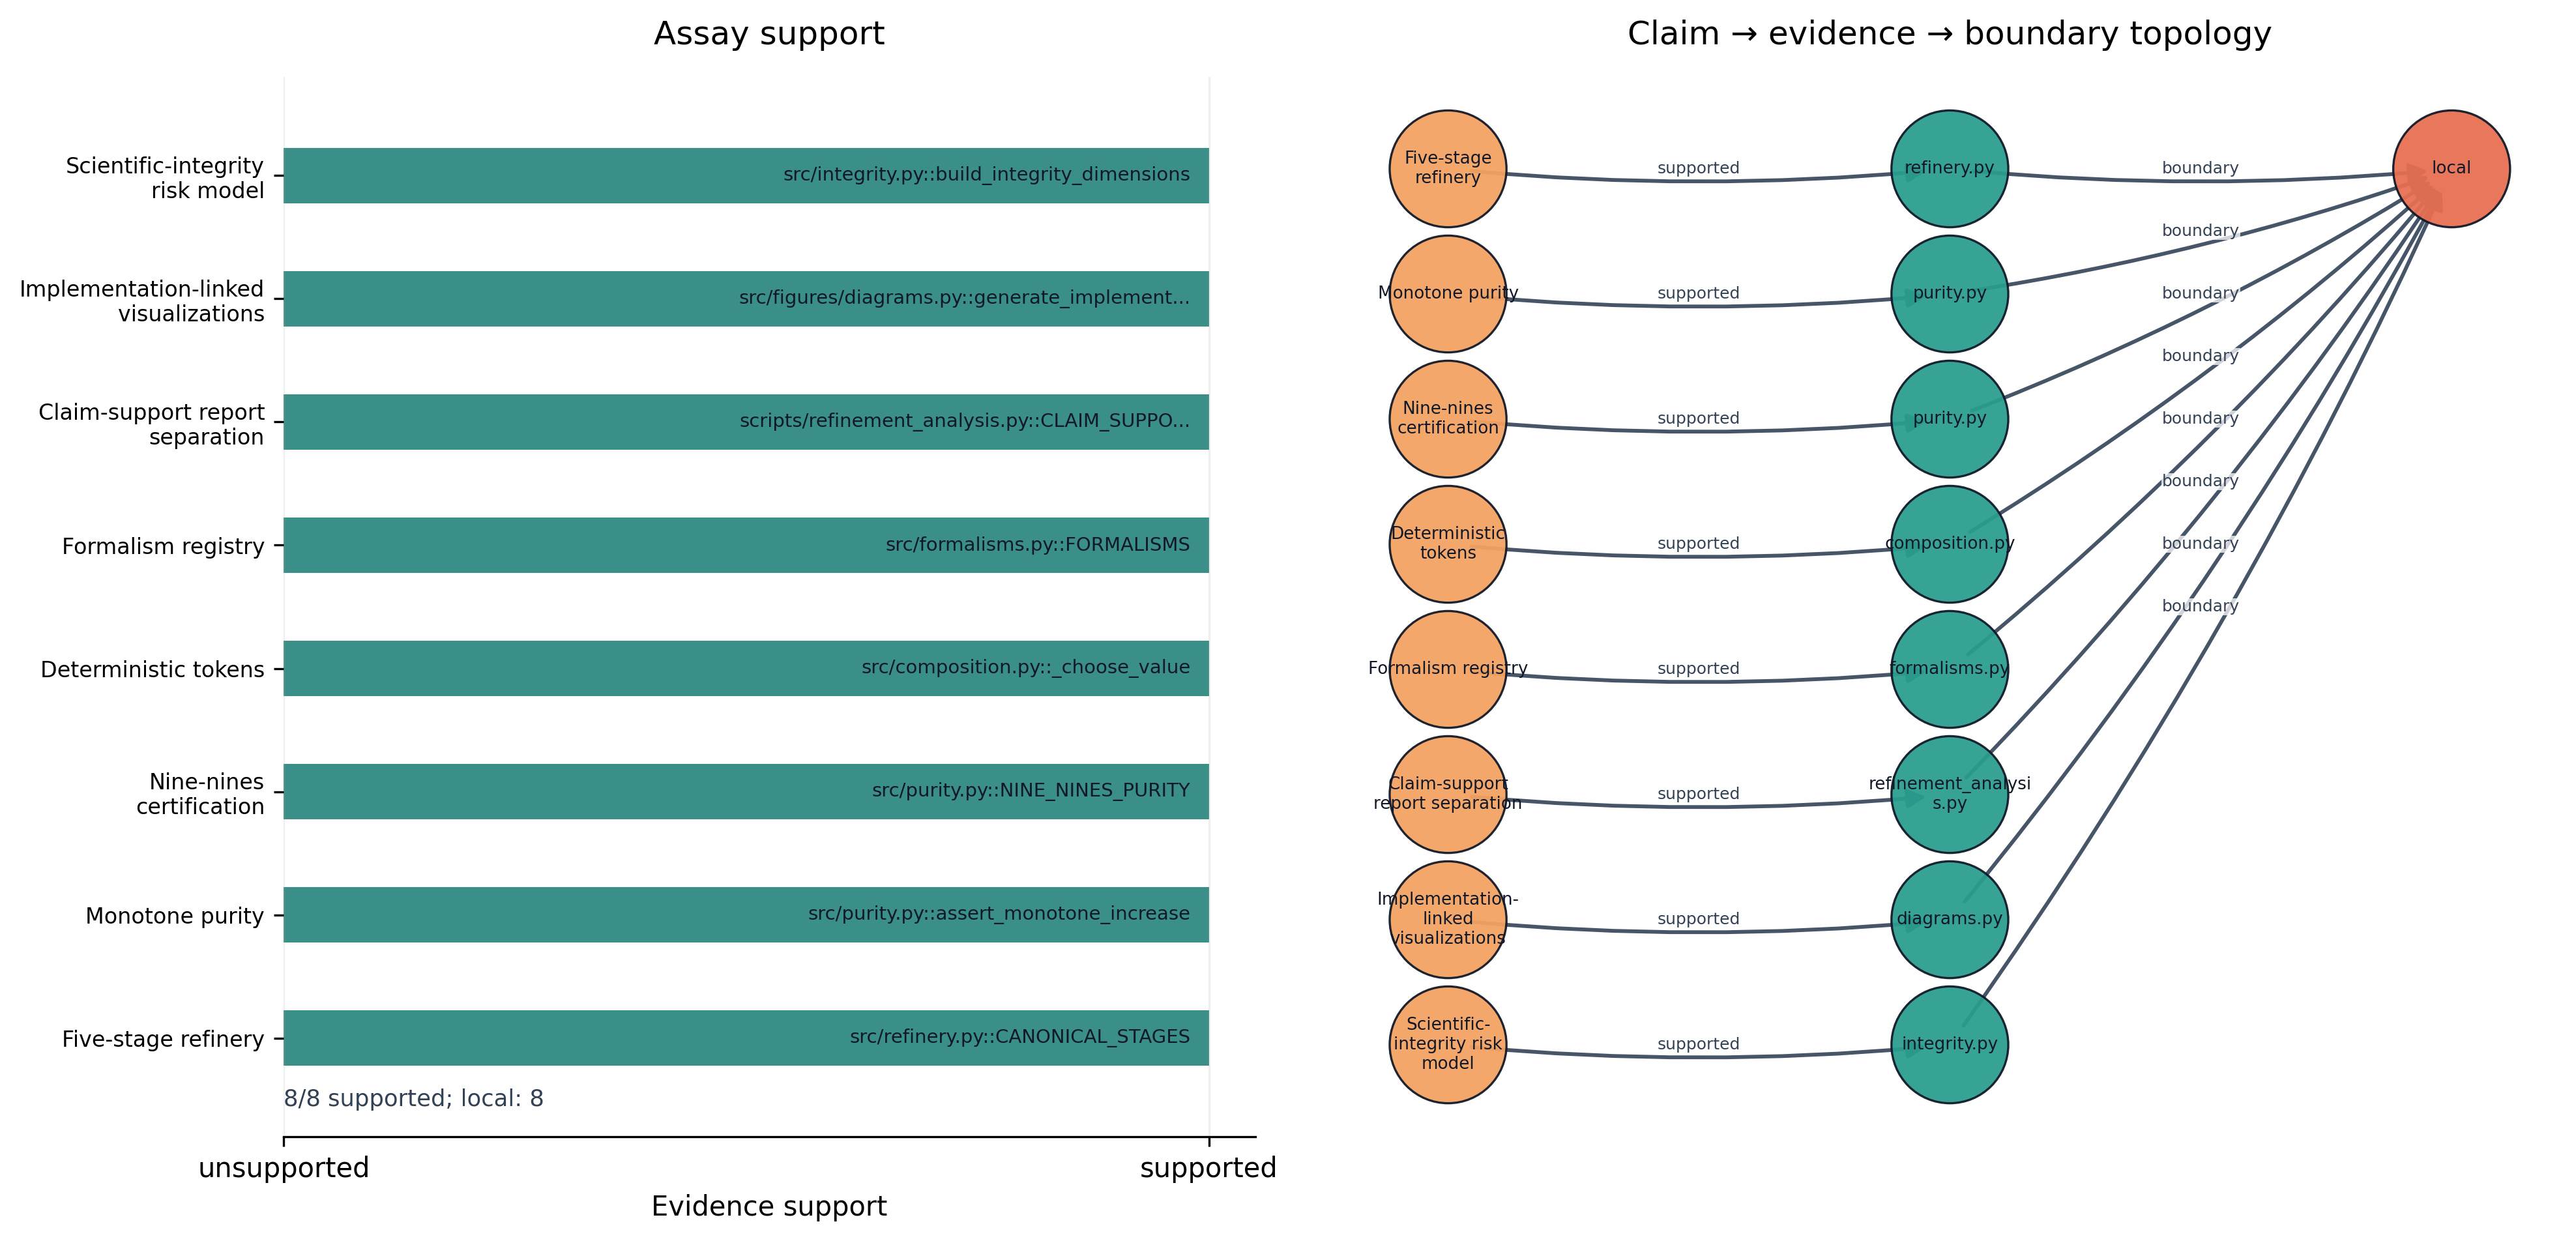
\includegraphics[keepaspectratio,alt={Claim-evidence assay}]{../figures/claim_evidence_assay.png}}
\caption{Claim-evidence assay}\label{fig:claim_evidence_assay}
\end{figure}

\subsection{Scientific-integrity risk
matrix}\label{scientific-integrity-risk-matrix}

The integrity risk matrix in fig.~\ref{fig:integrity_risk_matrix} plots
severity against detectability for the 8 integrity dimensions in
tbl.~\ref{tbl:integrity_dimensions}. Bubble size encodes residual risk,
while color encodes the source tier that owns the evidence surface. This
makes boundary failures more visible than cosmetic source checks without
hiding whether the support comes from config, source code, claim ledger,
generated metric, artifact, bibliography, or validation gate. The matrix
is intentionally local: it prioritizes where this exemplar needs source
ownership, not where every future manuscript should focus.

\begin{figure}
\centering
\pandocbounded{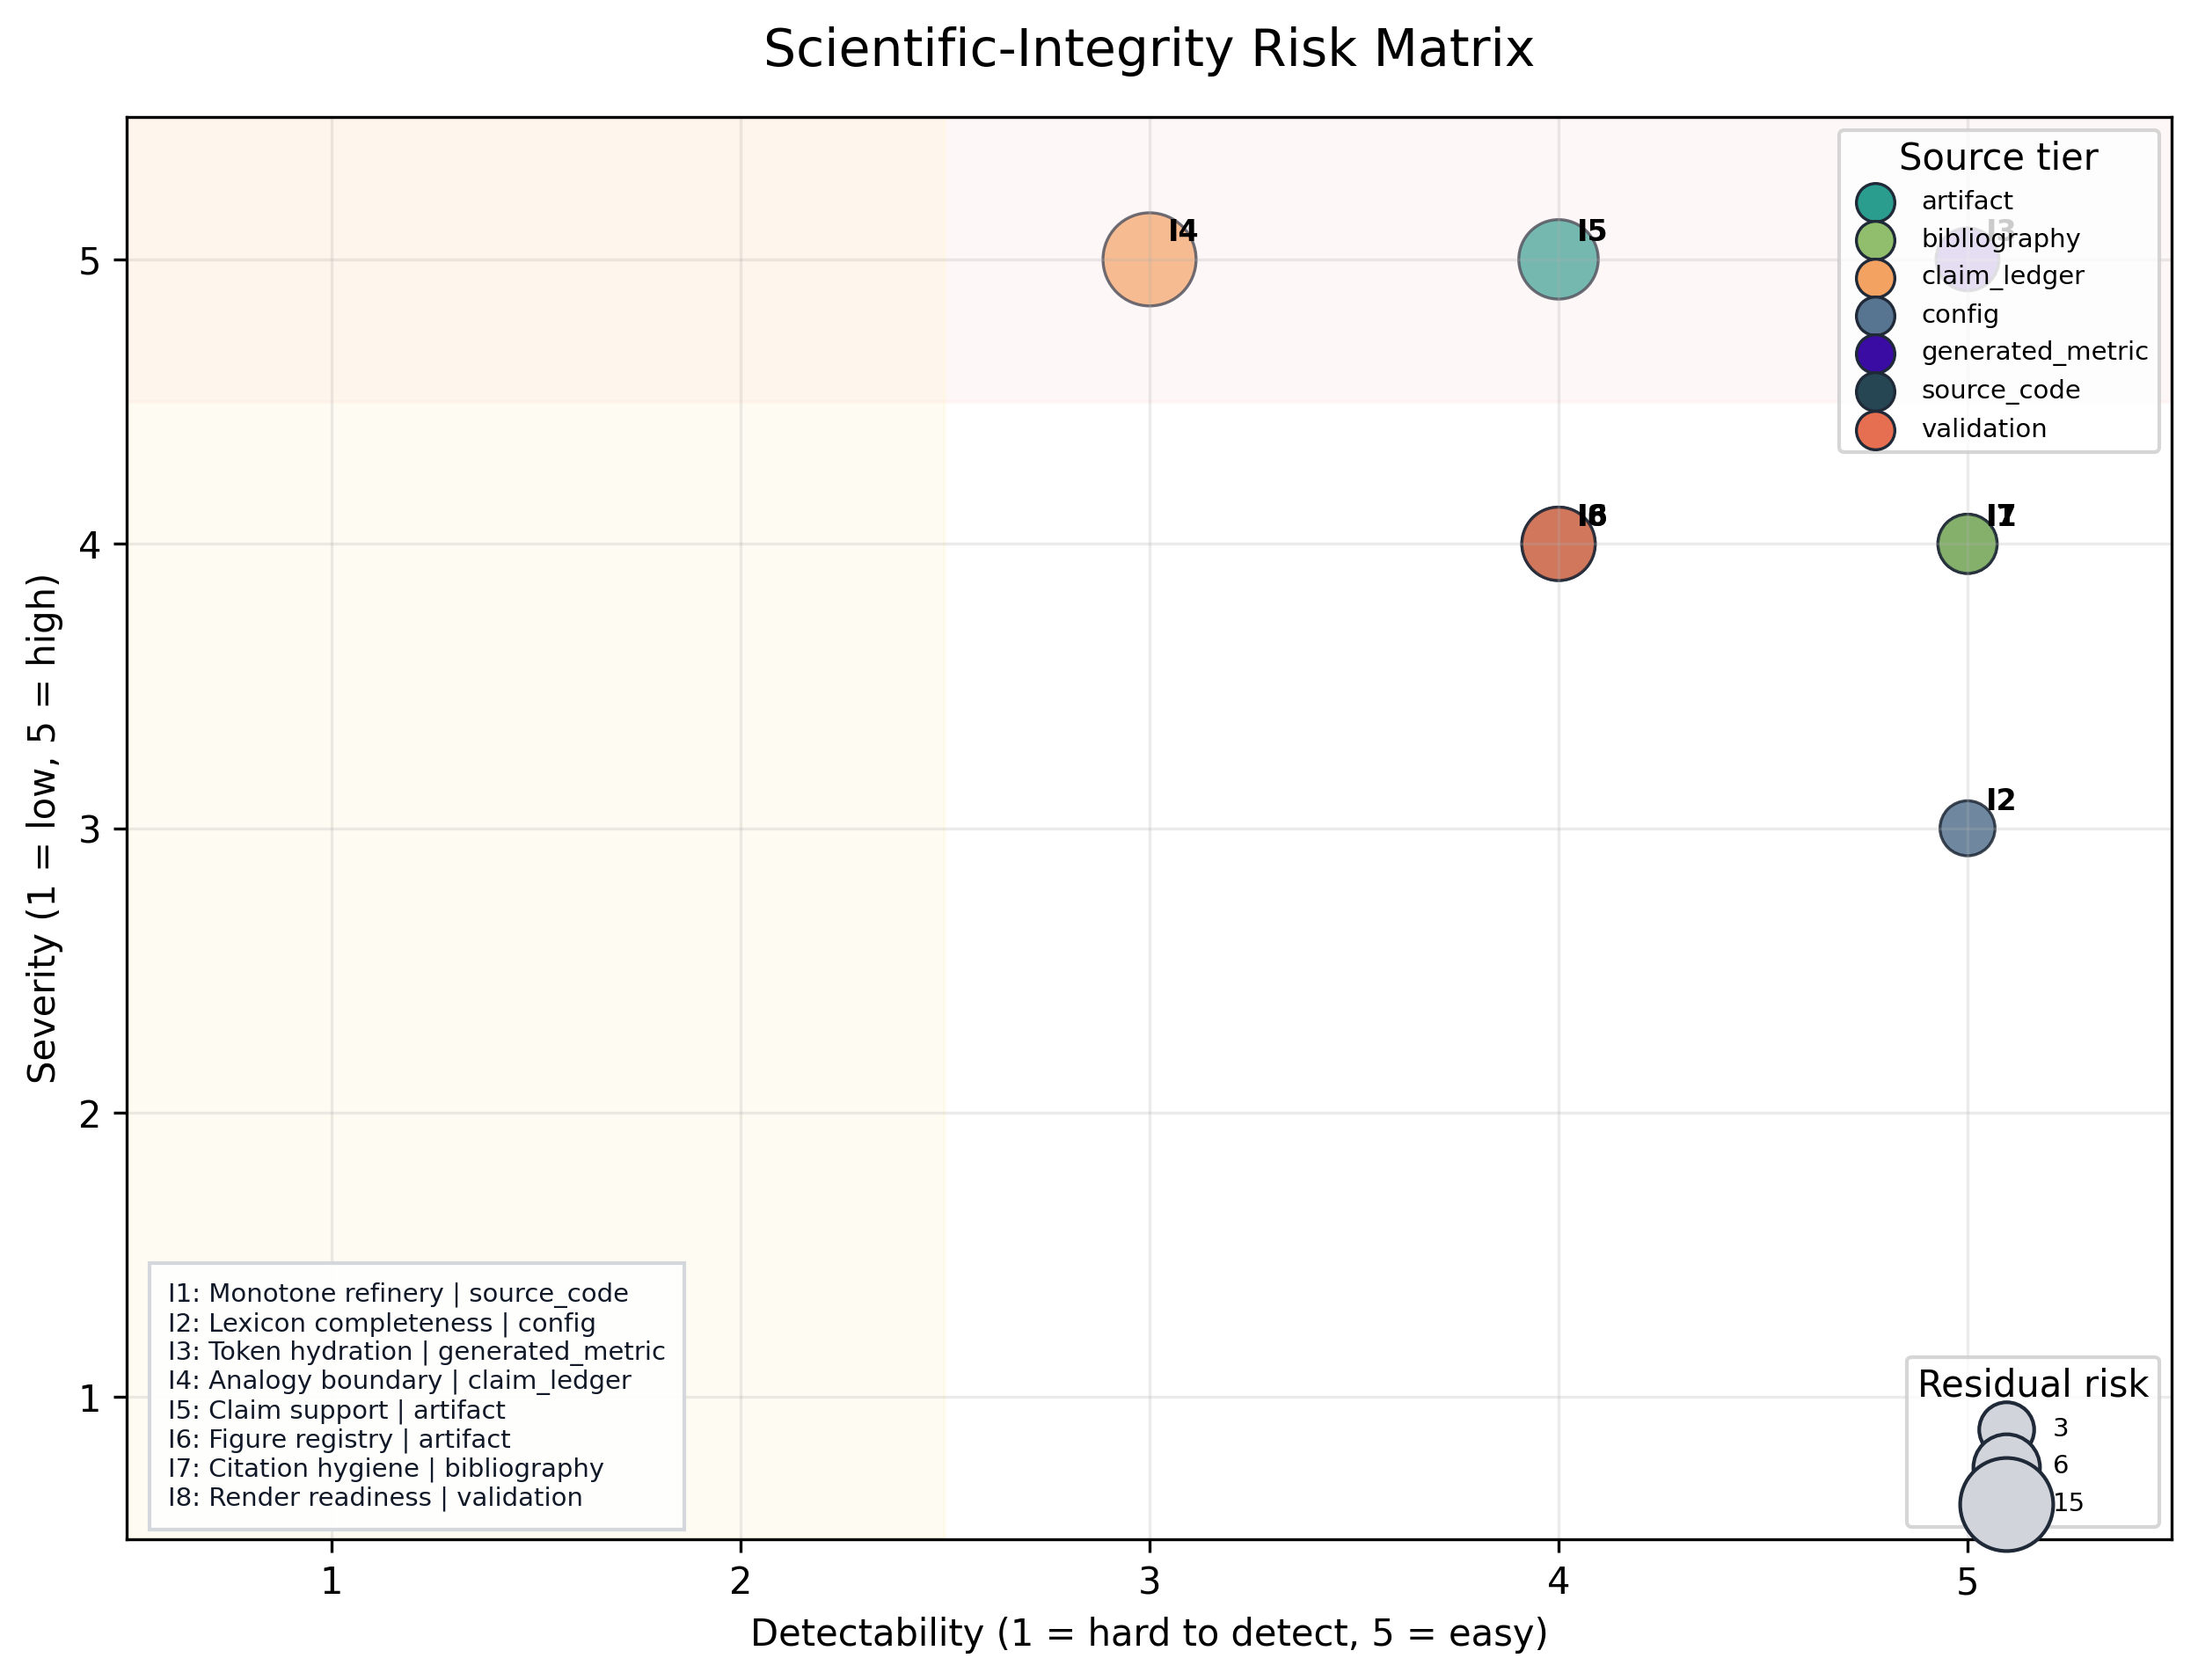
\includegraphics[keepaspectratio,alt={Scientific-integrity risk matrix}]{../figures/integrity_risk_matrix.png}}
\caption{Scientific-integrity risk
matrix}\label{fig:integrity_risk_matrix}
\end{figure}

\subsection{Evidence-tier ladder}\label{evidence-tier-ladder}

The evidence-tier ladder in fig.~\ref{fig:evidence_tier_ladder}
summarizes the evidence surfaces available to the shared template
evidence registry or, before that gate has run, the fallback source
tiers from the integrity model. It gives a quick view of whether the
manuscript is leaning on generated metrics, claim-ledger facts,
bibliography records, source code, or disposable artifacts.

\begin{figure}
\centering
\pandocbounded{
\includegraphics[keepaspectratio,alt={Evidence-tier ladder}]{../figures/evidence_tier_ladder.png}}
\caption{Evidence-tier ladder}\label{fig:evidence_tier_ladder}
\end{figure}

\begin{longtable}[]{@{}lll@{}}
\caption{Evidence tiers used by the integrity model and shared registry
when available.}\label{tbl:evidence_tiers}\tabularnewline
\toprule\noalign{}
Source tier & Count & Role \\
\midrule\noalign{}
\endfirsthead
\toprule\noalign{}
Source tier & Count & Role \\
\midrule\noalign{}
\endhead
\bottomrule\noalign{}
\endlastfoot
artifact & 117 & Generated artifacts exposed to readers \\
generated\_metric & 94 & Numbers regenerated from project analysis \\
claim\_ledger & 14 & Source-owned claim and fact declarations \\
bibliography & 5 & Reference records and citation metadata \\
\end{longtable}

\subsection{Contribution claims}\label{contribution-claims}

{\def\LTcaptype{none} % do not increment counter
\begin{longtable}[]{@{}
  >{\raggedright\arraybackslash}p{(\linewidth - 6\tabcolsep) * \real{0.1842}}
  >{\raggedright\arraybackslash}p{(\linewidth - 6\tabcolsep) * \real{0.2895}}
  >{\raggedright\arraybackslash}p{(\linewidth - 6\tabcolsep) * \real{0.2632}}
  >{\raggedright\arraybackslash}p{(\linewidth - 6\tabcolsep) * \real{0.2632}}@{}}
\toprule\noalign{}
\begin{minipage}[b]{\linewidth}\raggedright
Claim
\end{minipage} & \begin{minipage}[b]{\linewidth}\raggedright
Statement
\end{minipage} & \begin{minipage}[b]{\linewidth}\raggedright
Evidence
\end{minipage} & \begin{minipage}[b]{\linewidth}\raggedright
Boundary
\end{minipage} \\
\midrule\noalign{}
\endhead
\bottomrule\noalign{}
\endlastfoot
Five-stage refinery & The refinery pipeline has 5 canonical stages from
ore to nine-nines. & src/refinery.py::CANONICAL\_STAGES & local \\
Monotone purity & Purity increases strictly across all refinery stages.
& src/purity.py::assert\_monotone\_increase & local \\
Nine-nines certification & The certification stage achieves 99.9999999\%
purity. & src/purity.py::NINE\_NINES\_PURITY & local \\
Deterministic tokens & Token selection is deterministic via seeded
SHA-256 digest. & src/composition.py::\_choose\_value & local \\
Formalism registry & The manuscript exposes 6 source-owned formalisms
with equation labels. & src/formalisms.py::FORMALISMS & local \\
Claim-support report separation & The project-local contribution-claim
report is written to claim\_support\_registry.json. &
scripts/refinement\_analysis.py::CLAIM\_SUPPORT\_REGISTRY\_NAME &
local \\
Implementation-linked visualizations & The manuscript includes generated
visualizations that link the refinery analogy to source code, variables,
evidence, and validation gates. &
src/figures/diagrams.py::generate\_implementation\_circuit & local \\
Scientific-integrity risk model & The manuscript includes a source-owned
integrity risk model linking failure modes, validators, evidence
surfaces, and fork obligations. &
src/integrity.py::build\_integrity\_dimensions & local \\
\end{longtable}
}

The project-local claim-support assay reports 8 supported claims out of
8 total claims, for 100.00\% support. Unsupported claims: 0. The
generated project report path is
\breaktt{output/reports/claim\_support\_registry.json}; the shared
template evidence report remains
\breaktt{output/reports/evidence\_registry.json}.

\subsection{Shared evidence registry
summary}\label{shared-evidence-registry-summary}

When the template evidence gate has run, the shared registry supplies
source-tiered facts used by the evidence validator. Current fact count
available to this variable pass: 230.

\begin{longtable}[]{@{}ll@{}}
\caption{Shared evidence-registry fact kinds when
available.}\label{tbl:shared_evidence_kinds}\tabularnewline
\toprule\noalign{}
Fact kind & Count \\
\midrule\noalign{}
\endfirsthead
\toprule\noalign{}
Fact kind & Count \\
\midrule\noalign{}
\endhead
\bottomrule\noalign{}
\endlastfoot
artifact & 75 \\
citation & 5 \\
equation & 7 \\
figure & 27 \\
number & 100 \\
section & 10 \\
table & 6 \\
\end{longtable}

\subsection{Figure quality report}\label{figure-quality-report}

The visualization registry is paired with
\breaktt{output/reports/figure\_quality\_report.json}, a generated QA
report that checks PNG and SVG existence, file dimensions, nonblank
pixel mass, color variance, and registry parity. Current status: passing
with 12/12 registered figures passing and registry parity reported as
Yes. PNG remains the manuscript render path; SVG is the companion
technical artifact for inspection, reuse, and source-level debugging.
tbl.~\ref{tbl:figure_quality} summarizes the generated surface.

\begin{longtable}[]{@{}
  >{\raggedright\arraybackslash}p{(\linewidth - 12\tabcolsep) * \real{0.1379}}
  >{\raggedright\arraybackslash}p{(\linewidth - 12\tabcolsep) * \real{0.0862}}
  >{\raggedright\arraybackslash}p{(\linewidth - 12\tabcolsep) * \real{0.0862}}
  >{\raggedright\arraybackslash}p{(\linewidth - 12\tabcolsep) * \real{0.2069}}
  >{\raggedright\arraybackslash}p{(\linewidth - 12\tabcolsep) * \real{0.1724}}
  >{\raggedright\arraybackslash}p{(\linewidth - 12\tabcolsep) * \real{0.1724}}
  >{\raggedright\arraybackslash}p{(\linewidth - 12\tabcolsep) * \real{0.1379}}@{}}
\caption{Figure-quality report generated from source-owned figure
specs.}\label{tbl:figure_quality}\tabularnewline
\toprule\noalign{}
\begin{minipage}[b]{\linewidth}\raggedright
Figure
\end{minipage} & \begin{minipage}[b]{\linewidth}\raggedright
PNG
\end{minipage} & \begin{minipage}[b]{\linewidth}\raggedright
SVG
\end{minipage} & \begin{minipage}[b]{\linewidth}\raggedright
Dimensions
\end{minipage} & \begin{minipage}[b]{\linewidth}\raggedright
Nonwhite
\end{minipage} & \begin{minipage}[b]{\linewidth}\raggedright
Variance
\end{minipage} & \begin{minipage}[b]{\linewidth}\raggedright
Status
\end{minipage} \\
\midrule\noalign{}
\endfirsthead
\toprule\noalign{}
\begin{minipage}[b]{\linewidth}\raggedright
Figure
\end{minipage} & \begin{minipage}[b]{\linewidth}\raggedright
PNG
\end{minipage} & \begin{minipage}[b]{\linewidth}\raggedright
SVG
\end{minipage} & \begin{minipage}[b]{\linewidth}\raggedright
Dimensions
\end{minipage} & \begin{minipage}[b]{\linewidth}\raggedright
Nonwhite
\end{minipage} & \begin{minipage}[b]{\linewidth}\raggedright
Variance
\end{minipage} & \begin{minipage}[b]{\linewidth}\raggedright
Status
\end{minipage} \\
\midrule\noalign{}
\endhead
\bottomrule\noalign{}
\endlastfoot
claim\_evidence\_assay & yes & yes & 3952x1904 & 0.211 & 0.05901302 &
pass \\
evidence\_tier\_ladder & yes & yes & 3348x1332 & 0.196 & 0.05503309 &
pass \\
formalism\_traceability & yes & yes & 3315x1631 & 0.133 & 0.04262721 &
pass \\
implementation\_circuit & yes & yes & 2966x1845 & 0.068 & 0.02235231 &
pass \\
integrity\_gate\_matrix & yes & yes & 1832x1425 & 0.437 & 0.17560313 &
pass \\
integrity\_risk\_matrix & yes & yes & 2499x1910 & 0.387 & 0.01770377 &
pass \\
karat\_grading & yes & yes & 2961x1698 & 0.279 & 0.07300982 & pass \\
provenance\_sankey & yes & yes & 2850x1461 & 0.070 & 0.02178809 &
pass \\
purity\_claim\_scatter & yes & yes & 2340x1744 & 0.032 & 0.01428277 &
pass \\
purity\_progression & yes & yes & 3024x2125 & 0.182 & 0.03967814 &
pass \\
token\_density & yes & yes & 3289x1856 & 0.234 & 0.06699486 & pass \\
token\_heatmap & yes & yes & 2397x2399 & 0.627 & 0.12908659 & pass \\
\end{longtable}

\newpage

\section{Discussion: Load-Bearing vs Rhetorical
Analogy}\label{sec:discussion}

\subsection{Load-bearing vs
rhetorical}\label{load-bearing-vs-rhetorical}

The gold-refining analogy operates on two levels. \textbf{Rhetorically},
it provides a memorable framing for a methods paper: purity progression,
karat grading, and certification are vivid metaphors for manuscript
quality. \textbf{Operationally}, each stage maps to a real
template-infrastructure operation --- smelting to claim removal,
assaying to evidence validation, cupellation to cross-reference
resolution, and certification to full pipeline validation.

The analogy is smelting the manuscript: it performs the refinement it
describes. Its fork obligation is equally important. Gold refining can
model staged purification, but it cannot certify domain truth unless the
fork supplies a real domain validator and evidence source.

The added implementation and claim-assay figures sharpen that boundary.
They show that ``purity'' is not a free-standing aesthetic judgment. It
is a local statement about whether source-owned stages, generated
artifacts, claim ledgers, figure registries, and validation commands
agree. The figures therefore make a negative claim as important as the
positive one: when a fork lacks a validator, a ledger, or a source
artifact, the metaphor must stop at analogy and cannot be promoted to
certification.

\subsection{Useful adaptation cases}\label{useful-adaptation-cases}

\begin{itemize}
\tightlist
\item
  \textbf{Domain-specific refinement pipelines}: fork the exemplar and
  remap stages to domain operations (e.g., clinical evidence, legal
  citation, engineering specification).
\item
  \textbf{Purity measurement}: adopt the purity fraction and karat grade
  vocabulary for any staged quality process.
\item
  \textbf{Mega-madlib composition}: reuse the deterministic token engine
  for any config-owned lexical composition task.
\item
  \textbf{Domain adapters}: use \breaktt{src/domain\_adapter.py} and
  \breaktt{domain\_profile.yaml} to translate a domain's own metrics into
  the same purity scale before reusing certification language.
\end{itemize}

\subsection{Misuse modes}\label{misuse-modes}

{\def\LTcaptype{none} % do not increment counter
\begin{longtable}[]{@{}
  >{\raggedright\arraybackslash}p{(\linewidth - 6\tabcolsep) * \real{0.1714}}
  >{\raggedright\arraybackslash}p{(\linewidth - 6\tabcolsep) * \real{0.1714}}
  >{\raggedright\arraybackslash}p{(\linewidth - 6\tabcolsep) * \real{0.3143}}
  >{\raggedright\arraybackslash}p{(\linewidth - 6\tabcolsep) * \real{0.3429}}@{}}
\toprule\noalign{}
\begin{minipage}[b]{\linewidth}\raggedright
Mode
\end{minipage} & \begin{minipage}[b]{\linewidth}\raggedright
Risk
\end{minipage} & \begin{minipage}[b]{\linewidth}\raggedright
Detection
\end{minipage} & \begin{minipage}[b]{\linewidth}\raggedright
Mitigation
\end{minipage} \\
\midrule\noalign{}
\endhead
\bottomrule\noalign{}
\endlastfoot
Non-monotone purity & A stage has lower output purity than input. &
assert\_monotone\_increase raises ValueError. & Fix stage purity targets
in src/refinery.py. \\
Empty lexicon category & A required lexicon category is empty or
missing. & Config validation raises GoldRefinementConfigError. & Add
vocabulary to manuscript/config.yaml. \\
Unresolved token & A manuscript placeholder has no generated variable. &
test\_all\_manuscript\_tokens\_are\_generated fails. & Add variable in
src/manuscript\_variables.py. \\
Rhetorical-only analogy & The analogy is decorative with no operational
mapping. & Review that each stage maps to a real infrastructure
operation. & Connect stages to template pipeline operations. \\
Undetected integrity gap & A high-severity failure mode is present but
no owner, validator, or generated artifact makes it visible. &
build\_integrity\_dimensions lists severity, detectability, owner,
validator, and evidence surface. & Add or revise the source-owned
integrity dimension before promoting the manuscript. \\
\end{longtable}
}

\subsection{Design principles}\label{design-principles}

{\def\LTcaptype{none} % do not increment counter
\begin{longtable}[]{@{}
  >{\raggedright\arraybackslash}p{(\linewidth - 2\tabcolsep) * \real{0.5000}}
  >{\raggedright\arraybackslash}p{(\linewidth - 2\tabcolsep) * \real{0.5000}}@{}}
\toprule\noalign{}
\begin{minipage}[b]{\linewidth}\raggedright
Principle
\end{minipage} & \begin{minipage}[b]{\linewidth}\raggedright
Rationale
\end{minipage} \\
\midrule\noalign{}
\endhead
\bottomrule\noalign{}
\endlastfoot
Analogy is load-bearing & Each metallurgical stage maps to a real
template-infrastructure operation, not mere decoration. \\
Purity increases monotonically & The refinery pipeline guarantees
strictly increasing purity from ore to certification. \\
Token selection is deterministic & A fixed seed and lexicon produce the
same injection plan across reruns. \\
Configuration owns prose choices & Reviewers can inspect the declared
language surface before generation. \\
Generated output is disposable & The durable artifact is the
regeneration contract, not hand-edited output. \\
\end{longtable}
}

\subsection{Analogy-break boundary}\label{analogy-break-boundary}

The analogy breaks when purity becomes a rhetorical grade detached from
evidence. In this exemplar, eq.~\ref{eq:claim_support} and
eq.~\ref{eq:integrity_vector} keep the grade tied to claim support and
gate coverage. A fork that cannot provide comparable source-owned gates
should keep the gold-refining language as metaphor only and avoid
publication-strength claims.

The practical rule is simple: do not add an impressive figure unless its
path through fig.~\ref{fig:implementation_circuit} is visible. A visual
can summarize an idea, but it only supports a manuscript claim when the
claim-evidence assay can point to the owning file, symbol, generated
artifact, and validation surface.

The integrity risk matrix adds one more brake. A fork may have all
figures registered and still be scientifically weak if its
highest-severity risks are only weakly detectable. In this exemplar,
tbl.~\ref{tbl:integrity_dimensions} makes that weakness inspectable by
pairing each dimension with an owner and validator. The useful question
for a fork is therefore not ``can the manuscript render?'' but ``which
severe failures would the current pipeline miss, and what source-owned
gate would expose them?''

The evidence-tier ladder also prevents a common drift in generated
manuscripts: treating generated artifacts as if they were independent
evidence. A generated metric can support an internal consistency claim,
but a domain claim needs a domain source tier. The ladder makes that
distinction visible without pretending that a large fact count is the
same as stronger external validity.

\newpage

\section{Conclusion: Certification and Forking}\label{sec:conclusion}

The gold-refinery pipeline demonstrates that a metallurgical analogy can
be load-bearing: each stage maps to a real template-infrastructure
operation, purity increases monotonically, and the final stage achieves
nine-nines certification (99.9999999\% (nine-nines)).

\subsection{Summary}\label{summary}

\begin{itemize}
\tightlist
\item
  5 refinery stages from ore (9K) to certification (nine-nines)
\item
  Final purity: 99.9999999\% (nine-nines) (24K (nine-nines certified))
\item
  24 tokens generated deterministically from seed 431
\item
  Config hash: c0c52883efd82461
\item
  6 source-owned formalisms with equation labels: eq:purity\_functional,
  eq:monotone\_refinery, eq:token\_digest, eq:claim\_support,
  eq:integrity\_vector, eq:certification\_predicate
\item
  Claim-support status: 8/8 supported (passing)
\item
  8 integrity dimensions with residual-risk scoring and owner/validator
  links.
\item
  Registered visual evidence spans purity progression, token coverage,
  formalism traceability, implementation flow, claim-evidence assay,
  risk-matrix, and evidence-tier surfaces.
\end{itemize}

\subsection{Forking responsibilities}\label{forking-responsibilities}

\begin{enumerate}
\def\labelenumi{\arabic{enumi}.}
\tightlist
\item
  Remap metallurgical stages to domain operations
\item
  Update lexicon categories in \breaktt{manuscript/config.yaml}
\item
  Add domain-specific evidence and validators
\item
  Regenerate all outputs through the pipeline
\item
  Do not hand-edit generated manuscript, PDFs, or figures
\end{enumerate}

The durable result is not the current prose snapshot. It is the
reproducible contract that can rebuild the prose, figures, formalisms,
and validation reports from source.

That contract is the paper's central contribution. It demonstrates how
an analogy can be useful without being loose: every metaphorical move
either points to a source-owned implementation surface or stays
explicitly inside the discussion boundary.

The added integrity model makes the same claim in a stricter form: every
high-value visual or formal statement should have an owner, an evidence
tier, and a validator. Without those three surfaces, the right outcome
is not a more polished metaphor; it is a narrower claim.

\newpage

\section{Reproducibility: Seeded
Regeneration}\label{sec:reproducibility}

\subsection{Deterministic
regeneration}\label{deterministic-regeneration}

The refinery pipeline is fully deterministic. Given the same
\breaktt{manuscript/config.yaml} and \texttt{src/} code, every run
produces identical output.

\begin{itemize}
\tightlist
\item
  \textbf{Seed:} 431
\item
  \textbf{Config hash:} c0c52883efd82461
\item
  \textbf{Generation timestamp:} 2026-06-29T02:40:13Z
\item
  \textbf{Python version:} 3.12.13
\end{itemize}

\subsection{Artifact inventory}\label{artifact-inventory}

{\def\LTcaptype{none} % do not increment counter
\begin{longtable}[]{@{}ll@{}}
\toprule\noalign{}
Category & Count \\
\midrule\noalign{}
\endhead
\bottomrule\noalign{}
\endlastfoot
Figures & 24 \\
Data files & 3 \\
Reports & 11 \\
\textbf{Total} & 38 \\
\end{longtable}
}

\subsection{Regeneration commands}\label{regeneration-commands}

\begin{Shaded}
\begin{Highlighting}[]
\CommentTok{\# Run the refinery analysis}
\ExtensionTok{uv}\NormalTok{ run python projects/templates/template\_gold\_refinement/scripts/refinement\_analysis.py}

\CommentTok{\# Generate manuscript variables}
\ExtensionTok{uv}\NormalTok{ run python projects/templates/template\_gold\_refinement/scripts/z\_generate\_manuscript\_variables.py}

\CommentTok{\# Full pipeline (from repo root)}
\ExtensionTok{./run.sh} \AttributeTok{{-}{-}project}\NormalTok{ templates/template\_gold\_refinement }\AttributeTok{{-}{-}pipeline} \AttributeTok{{-}{-}core{-}only}
\end{Highlighting}
\end{Shaded}

\subsection{Config ownership}\label{config-ownership}

All vocabulary, slots, section conditions, steganography toggles, and
optional LLM review gates are declared in
\breaktt{manuscript/config.yaml} under \breaktt{gold\_refinement:},
\texttt{steganography:}, and \texttt{llm:}. The config is the source of
truth; generated prose is disposable.

\breaktt{src/pipeline\_policy.py} turns those policy blocks into an
explicit secure-pipeline hook. That keeps the optional hardening path
visible before execution instead of burying it in shell glue or prose.

The reproducibility spine uses fact registry and figure registry as
generated artifacts rather than reader trust signals. Variable
generation records \breaktt{c0c52883efd82461}; analysis writes refinery,
token, claim-support, dashboard, and figure artifacts; validation may
add the shared evidence registry used by template scientific-integrity
checks.

The implementation circuit gives a reproducibility checklist for future
forks. A reader should be able to start at any rendered figure or claim,
follow it to a generated variable or report, follow that artifact to
\texttt{src/} or \breaktt{manuscript/config.yaml}, and rerun the same
stage command. If that path is broken, the fork has produced a static
illustration rather than a reproducible refinement pipeline.

The same rule applies to visual polish. The figure registry is
source-owned, every registered PNG now has a companion SVG, and
\breaktt{output/reports/figure\_quality\_report.json} records 12 PNG
files, 12 SVG files, and 12 passing visual-quality checks for the
current variable pass. A fork should treat tbl.~\ref{tbl:figure_quality}
as the figure-layer analogue of the claim-support registry: it proves
that the visuals are regenerated, present in both raster and vector
forms, nonblank, and aligned with the registry before prose promotes
them.

\subsection{Evidence-registry
separation}\label{evidence-registry-separation}

This exemplar now separates two evidence surfaces.
\breaktt{output/reports/claim\_support\_registry.json} is the
project-local contribution-claim assay consumed by the dashboard and
claim-support figure. \breaktt{output/reports/evidence\_registry.json} is
reserved for the shared template evidence validator, which registers
numbers, citations, equations, sections, figures, tables, generated
data, and claim-ledger facts.

The evidence-tier ladder in fig.~\ref{fig:evidence_tier_ladder} is the
reproducibility counterpart to that separation. It does not merely count
files. It shows which tier owns each support surface, so a future fork
can see whether a conclusion rests on config declarations, generated
metrics, claim-ledger facts, bibliography records, or rendered
artifacts. That distinction matters because only some tiers can support
domain truth; others support reproducibility, formatting, or local
consistency.

\newpage

\section{Scope: Related Work and Limitations}\label{sec:scope}

\subsection{Scope limitations}\label{scope-limitations}

This exemplar demonstrates the gold-refining analogy as a
\textbf{methods paper}. It does not claim:

\begin{itemize}
\tightlist
\item
  Empirical validation of manuscript quality metrics against external
  standards
\item
  Generalizability of specific purity fractions to all scientific
  domains
\item
  That the analogy replaces domain-specific peer review or expert
  judgement
\end{itemize}

\subsection{Related work}\label{related-work}

The mega-madlib token injection pattern follows
\texttt{template\_madlib}'s deterministic lexical composition approach.
The pipeline-staging model draws on \breaktt{template\_code\_project}'s
thin-orchestrator pattern. The refinement analogy is novel to this
exemplar but builds on the template repository's existing validation and
rendering infrastructure.

\subsection{Responsible forking}\label{responsible-forking}

A fork must:

\begin{enumerate}
\def\labelenumi{\arabic{enumi}.}
\tightlist
\item
  Add domain-specific evidence before making domain claims
\item
  Update lexicon categories to reflect domain vocabulary
\item
  Connect refinery stages to real domain operations
\item
  Add domain validators beyond the exemplar's generic gates
\item
  Use \breaktt{src/domain\_adapter.py} and
  \breaktt{docs/domain\_fork\_guide.md} to remap domain metrics and
  boundary notes
\item
  Regenerate all outputs through the pipeline
\end{enumerate}

The formalism registry is local to this exemplar. It states how this
project maps refinery stages, token selection, and evidence gates into
equations; it does not prove that gold refining is a universal model of
scientific writing. Domain forks should replace or narrow the formalism
set before reusing the certification language.

The same limitation applies to the integrity risk model. The current 8
dimensions are tuned to a template exemplar: token hydration, figure
registration, claim support, citation hygiene, render readiness, and
analogy boundaries. A fork that studies a real domain must add
domain-specific risks, domain evidence tiers, and validators before
treating fig.~\ref{fig:integrity_risk_matrix} as a publication-readiness
claim.

\newpage

\section{Quality Probes}\label{sec:evaluation}

\subsection{QA probes}\label{qa-probes}

{\def\LTcaptype{none} % do not increment counter
\begin{longtable}[]{@{}
  >{\raggedright\arraybackslash}p{(\linewidth - 6\tabcolsep) * \real{0.1667}}
  >{\raggedright\arraybackslash}p{(\linewidth - 6\tabcolsep) * \real{0.2381}}
  >{\raggedright\arraybackslash}p{(\linewidth - 6\tabcolsep) * \real{0.3571}}
  >{\raggedright\arraybackslash}p{(\linewidth - 6\tabcolsep) * \real{0.2381}}@{}}
\toprule\noalign{}
\begin{minipage}[b]{\linewidth}\raggedright
Probe
\end{minipage} & \begin{minipage}[b]{\linewidth}\raggedright
Question
\end{minipage} & \begin{minipage}[b]{\linewidth}\raggedright
Passing signal
\end{minipage} & \begin{minipage}[b]{\linewidth}\raggedright
Artifact
\end{minipage} \\
\midrule\noalign{}
\endhead
\bottomrule\noalign{}
\endlastfoot
Monotone purity & Does purity increase strictly across all refinery
stages? & assert\_monotone\_increase passes on the purity sequence. &
src/refinery.py and output/data/refinery\_results.json \\
Token provenance & Can every selected token be traced to a category,
section, value, and config key? & The token plan contains one row for
each generated token. & output/reports/token\_plan.json \\
Karat grade correctness & Does each stage map to the correct karat
grade? & karat\_for\_purity returns the expected grade for each stage. &
src/purity.py \\
Integrity risk visibility & Can the manuscript identify high-severity
integrity failures and the validator or artifact that detects them? &
The integrity risk model emits dimensions, owners, residual risk scores,
and evidence-tier rows. & src/integrity.py and
../figures/integrity\_risk\_matrix.png \\
\end{longtable}
}

The selected evaluation gate terms are prerender and citation
validation. They are intentionally narrower than peer review: they check
source ownership, token coverage, figure registration, claim support,
and rendering integrity before a human reviewer assesses the substantive
analogy.

\subsection{Audit rules}\label{audit-rules}

{\def\LTcaptype{none} % do not increment counter
\begin{longtable}[]{@{}
  >{\raggedright\arraybackslash}p{(\linewidth - 4\tabcolsep) * \real{0.3158}}
  >{\raggedright\arraybackslash}p{(\linewidth - 4\tabcolsep) * \real{0.3684}}
  >{\raggedright\arraybackslash}p{(\linewidth - 4\tabcolsep) * \real{0.3158}}@{}}
\toprule\noalign{}
\begin{minipage}[b]{\linewidth}\raggedright
Rule
\end{minipage} & \begin{minipage}[b]{\linewidth}\raggedright
Check
\end{minipage} & \begin{minipage}[b]{\linewidth}\raggedright
Test
\end{minipage} \\
\midrule\noalign{}
\endhead
\bottomrule\noalign{}
\endlastfoot
Purity monotonicity & Purity must strictly increase from stage to stage
& tests/test\_refinery.py \\
Token determinism & Same seed and lexicon must produce same token plan &
tests/test\_composition.py \\
Token coverage & Every manuscript \{\{TOKEN\}\} must have a generated
variable & tests/test\_manuscript\_variables.py \\
Config validation & Invalid config must raise GoldRefinementConfigError
& tests/test\_config.py \\
Figure generation & All figure generators must produce non-blank PNGs &
tests/test\_figures.py \\
Integrity model coverage & Integrity dimensions must have unique IDs,
owners, validators, and evidence surfaces & tests/test\_integrity.py \\
\end{longtable}
}

The audit rules are summarized visually in
fig.~\ref{fig:integrity_gate_matrix} and algebraically in
eq.~\ref{eq:integrity_vector}. A failed audit rule should block
certification language even if the PDF renders.

The risk model adds prioritization to the gate list.
fig.~\ref{fig:integrity_risk_matrix} separates easy-to-detect
implementation failures from severe boundary failures that need clearer
ownership. This keeps the evaluation surface from becoming a checklist
of equally weighted boxes: token coverage, citation validity, claim
support, and render readiness all matter, but a high-severity
low-detectability failure should shape the next source edit before
cosmetic manuscript polish.

\newpage

\section{Authoring Contract}\label{sec:authoring_contract}

\subsection{Obligations}\label{obligations}

{\def\LTcaptype{none} % do not increment counter
\begin{longtable}[]{@{}
  >{\raggedright\arraybackslash}p{(\linewidth - 2\tabcolsep) * \real{0.4800}}
  >{\raggedright\arraybackslash}p{(\linewidth - 2\tabcolsep) * \real{0.5200}}@{}}
\toprule\noalign{}
\begin{minipage}[b]{\linewidth}\raggedright
Obligation
\end{minipage} & \begin{minipage}[b]{\linewidth}\raggedright
Requirement
\end{minipage} \\
\midrule\noalign{}
\endhead
\bottomrule\noalign{}
\endlastfoot
Domain validator & Add domain-specific evidence before making domain
claims beyond the exemplar. \\
Config ownership & Keep lexicon and slots in config.yaml, not in
generated prose. \\
Regeneration contract & Regenerate outputs through the pipeline, not by
hand-editing. \\
Risk review & Treat high-residual-risk integrity dimensions as fork
obligations before publication claims are expanded. \\
\end{longtable}
}

The authoring boundary tokens for this section are analogy boundary and
non-claim. They mark the point where an author must either add new
evidence and validators or lower the claim from certification to
analogy.

\subsection{Fork checklist}\label{fork-checklist}

\begin{enumerate}
\def\labelenumi{\arabic{enumi}.}
\item
  Remap metallurgical stages to domain operations in
  \texttt{src/refinery.py}
\item
  Update lexicon categories in \breaktt{manuscript/config.yaml} under
  \breaktt{gold\_refinement.lexicon}
\item
  Update \breaktt{contribution\_claims} with domain-specific evidence
  pointers
\item
  Add domain validators beyond the exemplar's generic gates
\item
  Replace or extend \breaktt{src/integrity.py} dimensions when the fork
  introduces new failure modes
\item
  Update \breaktt{domain\_profile.yaml}, \breaktt{src/domain\_adapter.py},
  and \breaktt{docs/domain\_fork\_guide.md} when the analogy is forked
  into a new domain
\item
  Keep \texttt{steganography} and \texttt{llm} policy blocks explicit
  when the secure pipeline or optional review path is used
\item
  Regenerate all outputs through the pipeline:

\begin{Shaded}
\begin{Highlighting}[]
\ExtensionTok{uv}\NormalTok{ run python scripts/refinement\_analysis.py}
\ExtensionTok{uv}\NormalTok{ run python scripts/z\_generate\_manuscript\_variables.py}
\end{Highlighting}
\end{Shaded}
\item
  Do not hand-edit generated manuscript, PDFs, or figures
\end{enumerate}

Do not hard-code equation, figure, or table numbers in prose. Use
\texttt{{[}@eq:...{]}}, \texttt{{[}@fig:...{]}},
\texttt{{[}@tbl:...{]}}, and \texttt{{[}@sec:...{]}} so the renderer
owns numbering and the tests can detect dangling references.

The authoring contract treats the risk matrix as a source checklist, not
as a retrospective dashboard. If a fork cannot name who owns a
high-severity integrity dimension, which validator detects it, and which
evidence tier supports it, the fork should lower the claim boundary
until that missing surface exists.



\clearpage

\bibliography{references}
\end{document}
